\documentclass[a4paper,12pt,oneside]{book}
%\usepackage{geometry}
%\usepackage{fancyhdr}
%\usepackage{amsmath,amsthm,amssymb }
\usepackage{graphicx}
%\usepackage{lipsum}
\usepackage[utf8]{inputenc}
%\usepackage{ngerman}
%\usepackage{parskip}
\usepackage{textcomp}
\usepackage{float}
\usepackage{hyperref}
\usepackage{placeins}

\setlength{\parskip}{0.2cm}

\hypersetup{
    pdfborder = {0 0 0},		
}

% Hurenkinder und Schusterjungen verhindern
\clubpenalty10000
\widowpenalty10000
\displaywidowpenalty=10000

\pagestyle{plain}

\title{Zeos Documentation Collection}
\author{Jan Baumgarten}
\date{\today}
%\overfullrule=2mm
\begin{document}
\maketitle
\tableofcontents

\chapter{Introduction}
This document is an effort to combine all the available Zeos documentation in one Manual.
It includes a tutorial as found on the Internet and several other pieces.
It is started in the hopes that it somehow will evolve into a kinda manual.

Currently all the documentation here is kinda outdated.
It is in the process of being compiled in one manual and then will be updated as time permits.
Parts that have been updated will be marked in the future.

The user documentation is intended to be at least some help to new Zeos users and help them getting started.

The developer documentation is here for historic interests and to be a guide on what to think about while working on a new developer documentation.
Also it should help to understand how Zeos was organized in the past and still is organized.

\part{Zeos user documentation}

\chapter{A ZEOS basics tutorial not only for Firebird ...}
This tutorial was originally written by Michael Seeger.

\section{Preface}
The ZeosLib DBOs 6.1.5 - With Delphi 7 and Firebird 1.5.
This little article shows how to access Firebird databases by using the ZEOS component Library in version 6.1.5 (including Patches 1\&2) and how to use these components in database applications.
It does not matter if you use the "real" SQL-Server or the embedded version which is restricted to local held databases.
A couple of examples (also migrated Delphi-BDE demos) shall explain how to use the ZEOS
components.

Although this article describes the usage of the ZEOS Library using Firebird, all the basics can be used with other SQL servers / databases that are supported by ZEOS.

Note: The Firebird Server can be downloaded from download section of
http://www.ibphoenix.com
http://www.firebirdsql.org

\section{The ZEOS Library}
The name "ZEOS" has no special meaning. The founders of ZEOS found that this name just sounded good.
Since that time the Library is called "ZEOS".

Generally we can say about the ZEOS Library that the developers are inteneded to
copy the functions and the behaviour of the corresponding BDE components as good
as possible.
The intention is to minimize the learning courve for developers who
migrate from BDE to ZEOS.
Of course there must have been made some compromises so that they are not a hundred percent compatible because the ZEOS components shall be applicable universally.

The ZEOS Library in version 6.1.5 consists of the following nine components
which shall be introduced in the following:
\begin{itemize}
\item TZConnection
\item TZQuery
\item TZReadOnlyQuery
\item TZUpdateSQL
\item TZTable
\item TZStoredProc
\item TZSQLProcessor
\item TZSQLMonitor
\item TZSQLMetadata
\end{itemize}

\section{Installing the ZEOS Library and additional stuff}

The installation of the ZEOS Library under Delphi 7 professional is not that complicated.
Once the current ZEOS version and all the patches (while writing this article it was library version 6.1.5 and the corresponding patches 1\&2) are downloaded and unzipped into a directory of your choice completely you only have to follow the installation instructions (note: Firebird does not need any additional DLL's, here!):

Open the delphi project group ZeosDbo.bpg from subdirectory packages\textbackslash delphi7 ZeosDbo.bpg and install
the following components in given order:
\begin{itemize}
\item ZCore.bpl
\item ZParseSql.bpl
\item ZPlain.bpl
\item ZDbc.bpl
\item ZComponent.bpl
\end{itemize}

Note: If there occur some errors while compiling that say that a certain dcu file could not be found then just add the subdirectory packages\textbackslash delphi7\textbackslash build to delphis library path.
All dcu files that are created while compilation are located here.

Attention: The client library of Firebird Server version 1.5.1 (not embedded!) was delivered as "gds32.dll" and not "fbclient.dll".
This causes trouble while accessing via ZEOS because the protocol "firebird1.5" assumes a DLL named "fbclient.dll".
A workaround is to copy the "gds32.dll" and rename this copy to "fbclient.dll".

\section{Basics: Transactions}
Some mandatory basics about transactions have to be told in order to understand how the TZConnection
component works internally and how to work with it.

In general: You only can have access to a database within the context of a valid ("running") transaction.
A transaction has to fulfill the following four characteristics that are known as ACID characteristics of a transaction.

Atomicity: All actions performed on a database have to be executed successfully.
If only one error occurs then the original state of the database has to be restored.
According to the principle "all or nothing".

Consitency: A transaction transfers a database from one consitent state to an other consistent state.
If an error occurs then the original state of the database has to be restored.

Isolation: A transaction has to be handled by the server as if it was the only one running.
This means it has to run indepently from other transactions.
A user must not notice the changes done by other users.

Durability: Changes in the dataset of a database that are caused by SQL statements that are executed between the start of a transaction and a COMMIT have to be fixed irrevocably.

Transactions encapsulate consecutive accesses on a database.
A database access may be of reading or writing nature (INSERT, UPDATE, DELETE) or it may change the structure of a database.
Transactions are terminated by COMMIT or ROLLBACK.
COMMIT confirms all changes in a database since the start of a transaction.
ROLLBACK resets all changes in a database since the start of a transaction.

Transactions running on the server have to be isolated from each other.
So they may run independently.
A transaction has to be handled by the server as it was the only one that is currently running.
This means for the user that he must never see the changes of other users while he is in a running transaction because the other changes have nothing to do with his transaction.
This is called the isolation of a transaction.
By using different transaction isolation levels (TILs) the developer may protect the data of an SQL resultset from access by other transactions.
The behaviour described above is called the standard isolationlevel known as SERIALIZABLE.
The standard isolationlevel of Firebird is called SNAPSHOT and comes very close to SERIALIZABLE.

\section{The Zeos Components}

\subsection{TZConnection}
The TZConnection component is a combination of a BDE TDatabase like component a component that
handles a transaction.
This combination makes sense because all access to a Firebird database (and also other databases) is always made in a running transaction.
Such a transaction is startet by the ZEOS Library whenever a connection (method Connect of TZConnection) to a database is opened.
This causes that each database access is done within the context of a running transaction, automatically.
The so called AutoCommit mode is always on (set to "True").
This is also the standard behaviour of the corresponding BDE component.
If AutoCommit is activated then every change of an SQL statement will be confirmed in the database by COMMIT after its successful execution.
If this behaviour shall be turned off and an explicit transaction shall be started then the method StartTransaction has to be called.
Within this explicit transaction it is possible to execute a couple of SQL statements that make changes to the database, in succession.
These statements then can be confirmed as a "group" by COMMIT.
If an explicit transaction is active then AutoCommit is always turned off.
By Calling the Method Commit all the changes made within this explicit transaction are confirmed.
Calling the method Rollback resets these changes.
In both cases AutoCommit will be set to True when the method call (Commit or Rollback) is done.
The explicit transaction has ended.

\subsubsection{Retaining}
After confirming the chanes made in a transaction by COMMIT or resetting them by ROLLLBACK the
transaction normally is going to be ended and an existing resultset of a query or stored procedure will be discarded.
These COMMITs and ROLLBACKs are called "hard" commit or "hard" rollback.
By using the ZEOS library this will become a little bit different.
ZEOS keeps the resultset alive.
This is achieved by closing transaction with "soft" commits or "soft" rollbacks.
All this is done by the TZConnection object.
This method is called retaining.
The COMMIT and ROLLBACK commands are executed with the addition RETAINING.
Retaining causes the closing of the current transaction and immediately opening a new transaction with all the data and resources (especially the resultset) of the "old" transaction.

Retaining becomes a problem if it is uses for huge tables.
It constrains the internal cleanup mechanism of firebird (garbage collection).
This leads (because of the versioning and the multigenerational architecture of Firebird) to a lot of old records that have to be kept but will not be needed anymore.
This influences the server's performanced in a negative way.
A so called sweep would discard these old versions and improve the performance.
This sweep will only be executed by sending a "hard" COMMIT or ROLLBACK.
The ZEOS Library only executes these "hard" commands when ending the database connection (closing connection).
It is not possible to send them while a database connection is active. So the database connection should be deactivated and immediately activated occasionally to achieve this performance improvement.

\subsubsection{Transaction Isolation Levels of TZConnection}

The TZConnection component provides four useful and predefined Transaction Isolation Levels (TIL):

tiRepeatableRead:
It corresponds to the TIL "SNAPSHOT" which is the standard of Firebird servers.
It is a combination of the trasaction parameters "concurrency" and "nowait".
A snapshot of the current database is made.
Other users are only influenced (constrained) if two transactions work on one record simultaneously.
If conflicts arise while accessing data an error message will be returned.
Changes within other transactions will not be noticed.
This TIL covers the requirement of the SQL standard (SERIALIZABLE) widely.

tiReadCommitted:
It corresponds to the TIL "READ COMMITTED".
It is a combination of the transaction parameters "read\_committed", "rec\_version" and "nowait".
This TIL recognizes all changes in other transaction that have been confirmed by COMMIT.
The parameter "rec\_version" is responsible for the behaviour that the most current values that were committed by other users will be considered.
The parameter "nowait" is resposible for the behaviour that there is no waiting for the release of a locked record.
So the server is more stressed than in TIL tiRepeatableRead because it has to do all the refreshes to get these values again and again.

tiSerializable:
It corresponds to the TIL "SNAPSHOT TABLE STABILITY".
It is used to get an exclusive access to the result set.
Realized by transaction parameter "consistency" it prevents that "foreign" transaction may access the written data.
Only the transaction which has written the data may access them.
This prevents also a multi user access to the written data.
Because this TIL is very restrictive by accessing written data it should be applied with caution and care.

tiNone: No TIL is used to isolate the transaction.

The TIL tiReadUncommitted is not supported by Firebird.
If this TIL is used, an error will be triggerded and the transaction will not be isolated (like using tiNone).

\subsubsection{Recommendation}
It is advisable to isolate transactions with transaction isolation level tiRepeatableRead (the Firebird standard).
This TIL covers the requirement of the SQL standard (SERIALIZABLE) widely.
It prevents all problems concerning consistency that may arise by using transactions.
Second choice would be tiReadCommitted but this depends on the application and the necessity if the reseult set always has to be current.

\subsubsection{Customizing TILs}

If you want to customize your TILs or expand a given TIL then you can do this by using the parameters of TZConnection.
The most important thing about this is that the TIL that should be expanded has to be set in
property IsolationLevel.
If it is set the TIL parameters (see IB/FB API reference) you want to add may be added in sourcecode.
The following example shows the expansion of a TIL preset to tiNone:
\begin{verbatim}
ZConnection.TransactIsolationLevel := tiNone;
ZConnection.Properties.Add('isc_tpb_concurrency');
ZConnection.Properties.Add('isc_tpb_wait');
ZConnection.Connect;
\end{verbatim}

\subsubsection{Protocol}
The most important setting in a TZConnection object is the server protocol it is set in property Protocol.
It determines which protocol shall be used and thus which SQL server will be accessed.
This method makes ZEOS so flexible.
You don't have to install special components for each database you want to access as it was in Versions 5.x and earlier.
The components will be installed once.
This is enough.
You only choose the protocol for the supported SQL server you want to access and you are done.
So you set protocol "firebird1.5" to access Firebird 1.5 server.

\subsubsection{Read-Only-Connection}

The database connection maintained by a TZConnection object is set to read only by default (ReadOnly = True).
This means that no writing access to the connected database is allowed.
To get writing access to the database you have to set ReadOnly to False.

\subsubsection{Codepages}
Codepages will be determined by setting parameter "lc\_ctype" or "Codepage" in TZConnection.
This parameter must be added to the property Properties. E. g.:
\begin{verbatim}
ZConection.Properties.Add ('lc\_ctype=ISO8859\_1');
\end{verbatim}
or
\begin{verbatim}
ZConnection.Properties.Add ('Codepage=ISO8859\_1');
\end{verbatim}

Note: The Codepage support of Firebird (also embedded version) in version 1.5 with ZEOS is a little bit buggy. These bugs are corrected in Firebird version 1.5.1.

\subsubsection{Features of the Firebird embedded server}

Normally the server name or IP address of the server is given in property HostName.
By using a Firebird embedded server you may leave this property empty.
Only property Database has to be determined.
Here you have to specify drive path and name of the database including extension.

An other feature of the embedded server is that you may specify any login name with a pasword of your choice.
It doesn't matter what you choose you will get connected.

Setting the TZConnection object property Connected to True in designtime is extremely bad if you don't reset it to False before compiling.
If you then start the compiled application with IDE running you will get an error that says that the database cannot be opened because it is already in use.
So you should establish the connection to the database when starting the application (e. g. in OnCreate event of the main form) and then open the needed queries and tables.
Deactivating the connection should also be done in main form (e. g. in OnDestroy).
It is not necessary to close all open queries and tables.
This will be done when closing the connection of the TZConnection object.
If you use datamodel forms you have to take care that the datamodel form is created before the main form is created (set in the IDE's project options)...

\subsubsection{Useful TZConnection parameters}

Additional parameters for establishing connections to Firebird databases are:

CreateNewDataBase:
A new database will be created based on the specified CREATE DATABASE statements.
When the database is created the connection will be established immediately.
All this happens by calling the Connect method of TZConnection.
\begin{verbatim}
ZConnection1.Database := 'd:\db1.fdb';
ZConnection1.Protocol := 'firebird-1.5';
ZConnection1.Properties.Add ('CreateNewDatabase=CREATE DATABASE ' + QuotedStr ('d:\db1.fdb') + ' USER ' + QuotedStr ('sysdba') + ' PASSWORD ' + QuotedStr ('masterkey') + ' PAGE\_SIZE 4096 DEFAULT CHARACTER SET ISO8859\_1');
ZConnection1.Connect;
\end{verbatim}

To execute this correctly you have to set the Database and Protocol properties at minimum (also possible in objectinspector).

Dialect:
This parameter sets Firebird's SQL dialiect. To set dialect "1" you have to use the following code:
\begin{verbatim}
ZConnection.Properties.Add ('Dialect=1');
\end{verbatim}

The dialect of Firebird 1.5.x is set to "3" by default.

Rolename:
This parameter sets a rolename. A logged in user then works in the context of the role's rights but before the user has to be assigned to this role.
The Firebird embedded server does not support this feature.

\subsection{TZQuery}

The usage of TZQuery is similar to the usage of BDE's TQuery component.

\subsubsection{Recommandation: RequestLive and TZUpdateSQL}
If an SQL dataset shall be updatable then RequestLive has to be set to true and you should generally use according update SQL statements that will be defined in TZUpdateSQL.
If this is done just assign TZUpdateSQL to the TZQuery object.
Now all changes that will be made in the result set will be done to the database by using the defined statements of TZUpdateSQL.
According to experience RequestLive mode runs more smoothly by using TZUpdateSQL.

\subsubsection{Usage of parameters in SQL statements}

Using parameters in SELECT statments is as easy as using them with BDE's TQuery.
If TZQuery has a result set then you have to use the Open method.
If you want to execute an SQL statement which has no result set (e. g.: INSERT or UPDATE) you have to use ExecSQL (see also: TZStoredProc).

\subsection{TZReadOnlyQuery}

This is a Query component that is quite similar to the TZQuery component.
There is just one difference:
The result set is read only.
There is no possibility to assign a TZUpdateSQL object.

\subsection{TZUpdateSQL}

A TZUpdateSQL object provides statements to modify the data of a result set that is retrieved by a TZQuery object.
The TZUpdateSQL component is comparable to BDE's TUpdateSQL component.
Here is an example how to define the statements of an SQL statement with corresponding update statements (based on a dialect 3 database):

SQL: SELECT * FROM names

UpdateSQL.InsertSql: INSERT INTO names (recno, name) VALUES (:recno, :name)

UpdateSQL.ModifySql: UPDATE names SET recno = :RecNo, name = :name WHERE recno = :old\_recno

UpdateSQL.DeleteSql: DELETE FROM names WHERE recno = :old\_recno

\subsubsection{The "OLD\_" parameter prefix for SQL statements}

The "old\_" prefix is handled according to the handling with BDE components.
By using "OLD\_" as prefix for a fieldname you are able to access the value of the field before it was changed.
This is very helpful if you have to compare fieldvalues in a WHERE clause.

\subsubsection{Queries with read only resultsets}
In geneal a TZUpdateSQL object is assigned to a TZQuery object that has a read only resultset.
This makes it possible to change its data.
Such read only queries are queries that join multiple tables.
But also with "normal" "RequestLive" resultsets you may use TZUpdateSQL (see: TZQuery).

\subsubsection{Multiple statements in TZQuery and TZUpdateSQL}
The components TZQuery and TZUpdateSql provide the possibility to execute multiple statements, internally.
So it is possible to place multiple SQL statements (even with parameters) for execution in SQL property.
They only have to be separated by semicolon. Here an example:
\begin{verbatim}
:
With Query do Begin
Sql.Clear;
Sql.Add('DELETE FROM table1;');
Sql.Add('INSERT INTO table1 VALUES (:Val1, :Val2);');
Sql.Add('INSERT INTO table2 VALUES (:Val3, :Val2);');
Sql.Add('UPDATE table3 SET field1 = :Val4;');
Params.ParamByName('Val1').AsInteger := 123;
:
ExecSql;
End;
:
\end{verbatim}

The statements will be executed in given order.
It is also possible to execute multiple statements if they are grouped in this manner inside multiple TZUpdateSqlObjects in order to update multiple tables.

\subsection{TZTable}
TZTable acts like BDE's TTable.
As a principle you only should use TZTable in a C/S application if you have very small tables because all records of the table will be transferred from server into client's memory by
opening the TZTable.
This is a bahaviour similar to a "SELECT * FROM XYZ" statement.
You should even prevent a statement like this in a C/S application.
The intension is to keep the resultset that has to be transferred from server to client as small as possible (perferably onle one record).

\subsection{TZStoredProc}
TZStoredProc provides the possiblity to execute stored procedures that are saved in a database.
There are two kinds of stored procedures: Procedures that return a resultset and procedures that do not return a resultset.
TZStoredProc works similar to BDE's TStoredProc.
The only difference between them is that you don't have to call Prepare before you call the ExecProc method.

\subsubsection{Stored Procedures with Resultsets}

If a stored procedure returns a result set then it will be activated by calling the Open method (when all existing parameters have got their values):

\begin{verbatim}
:
With spSumByName do Begin
Close;
ParamByName ('Name').Value := 'DontKnowHow';
Open;
End;
:
\end{verbatim}

The resultset can be worked on like a resultset of a TZQuery.

\subsubsection{Stored Procedures without Resultsets}

If a stored procedure has no resultset then it will be executed by calling the ExecProc method (when all existing parameters have got their values).
Here is an example (conConnection.AutoCommit = True):

\begin{verbatim}
:
With spDeleteByName do Begin
  ParamByName ('Name').Value := 'DontKnowHow';
  conConnection.StartTransaction
  Try
    // execute StoredProc
    ExecProc;
  Except
    conConnection.Rollback;
  End;
  conConnection.Commit;
End;
:
\end{verbatim}

\subsubsection{Problems with TZStoredProc when using dialect 1 databases}
The problem when using dialect 1 databases is that the metadata of stored proecedure is not properly
transferred to the TZStoredProc objects when choosing the stored procedure in object inspector.
All parapeter data is not properly interpreted.
An update from dialect 1 to dialect 3 solves this problem.
Is the dialect 1 database vital for the application system then a TZQuery or TZReadOnlyQuery has to be used as workaround.

\subsection{TZSQLMonitor}
Using the TZSQLMonitor component you may log certain actions or events of the ZEOS database
components. The journal may be written as file or collected in a TMemo object or something like that.

Writing the actions or events to a logfile only needs a few settings:

\begin{verbatim}
:
sqlMonitor.FileName := 'C:\Log\MyAppLog.log';
sqlMonitor.Active := True;
sqlMonitor.AutoSave := True;
:
\end{verbatim}

To collect the logged actions or events in a TMemo object you have to implement the OnLogTrace event as
follows:

\begin{verbatim}
Procedure Tfrm_MyApp.sqlMonitorLogTrace (Sender: TObject; 
  Event: TZLoggingEvent);
Begin
  If Trim (Event.Error) > '' Then
    memMontor.Lines.Add (DateTimeToStr (Event.Timestamp) + ': ' 
		      + Event.Message + #13#10 + ' Error: ' + Event.Error)
  Else
    memMontor.Lines.Add (DateTimeToStr (Event.Timestamp) + ': ' 
		      + Event.Message);
End; // sqlMonitorLogTrace
\end{verbatim}

The OnLogTrace event is always triggered when an action or event was logged by sqlMonitor.LogEvent(oEvent).
The oEvent parameter stands for an instance of a TZLoggingEvent class object.

\subsubsection{Properties of TZLoggingEvent}
Category (TZLoggingCategory): Stands for the category of the logged action or event (lcConnect,
lcDisconnect, lcTransaction, lcExecute or lcOther)

Protocol (String): The protocol that is used to access the database (see: TZConnection)

Message (String): The text that is logged.

ErrorCode (Integer): The error code in case of an error.

Error (String): The error text in case of an error.

Timestamp (TDateTime): Date and time of the logged action or event.

\subsection{TZSQLMetadata}
With this special TDataSet component it is possible to access the metadata of a database like tables, columns, etc.
(This chapter is still to be expanded!)

\subsection{TZIBEventAlerter}
By using this component you are able to intercept events triggered by stored procedures of a Firebird
database and react to them.
You only have to register the event's text (string) you want to react to in property Events which is a stringlist.
You can do this using objectinspector or inside the sourcecode.
The event alerter is activated by registering the listed events.
To do this you should call the Registerevents method because the Properties AutoRegister and Registered do not work properly.
If you once have registered the events the component is able to react to them.
All events are unregistered (deleted) by calling method UnregisterEvents and the event alerter is turned off.

Registration of events and "activation" of the event alerter:

\begin{verbatim}
:
EventAlerter.Events.Add ('Minimum Stock Level Reached');
EventAlerter.Events.Add ('Credit Limit Exceeded');
EventAlerter.RegisterEvents;
:
\end{verbatim}

\section{Master/Detail with ZEOS Library}
ZEOS DataSet components come with two kinds of master/detail connections:
those with a server sided filter and those with a client sided filter.
Both kinds and one kind in additioin that is independent from ZEOS (and thus without any comfort) will be described here.

Note: If we talk about "master" or "detail" then a TDataSet descendant (TZQuery/TZReadOnlyQuery, TZTable or a TZStoredProc) is meant that accesses either a master resultset or a detail resultset of a master/detail connection.

\subsection{Master/Detail with server sided filters}
This method is the default behaviour of the BDE's TQuery component.
A master/detail connection of two DataSets is established as follows:

\begin{itemize}
  \item The master's DataSource is assigned to the DataSource of the detail.
	\item All primary key fields of the master have to be compared with the foreign key fields of the detail in the detail SQL statement.
\end{itemize}

This is an example for a simple master/detail queries. Requirement: We use TZQuery or TZReadOnlyQuery to establish the master/detail connection:

\begin{itemize}
\item Master SQL:
\begin{verbatim}
SELECT id, feld1, feld2, feld3
FROM master
\end{verbatim}

\item DetailSQL:
\begin{verbatim}
SELECT feld1, feld2, master_id
FROM detail
WHERE master_id = :id
\end{verbatim}
\end{itemize}

Parameter :id stands for the content of master's "id" field (is the primary key) because the master's DataSource is assigned to the property DataSource of the detail.
So this parameter references to the "id" field of the master.
The field "master\_id" in detail query is the foreign key field of the detail table which references the primary key of the master.

If the cursor of the master changes its position while server sided filters are used, the SQL statement of the detail is executed using the current key values.
So the result set of the detail is automatically refreshed.

\subsection{Master/Detail with client sided filters}
This is the default behaviour of a BDE TTable component.
Here a master/detail connection between two DataSets is established as follows:

\begin{itemize}
  \item The DataSource of the master is assigned to the property MasterDataSource of the detail.
	\item The primary key fields of the master are assigned to property MasterField of the detail.
	\item The foreign key of the detail which references the primary key of the master is assigned to propety IndexFieldNames.
\end{itemize}

This is an example for a simple master/detail queries.
Requirement: We use TZQuery or TZReadOnlyQuery to establish the master/detail connection:

\begin{itemize}
  \item Master SQL:
	  \begin{verbatim}
SELECT id, feld1, feld2, feld3
FROM master
    \end{verbatim}
  \item DetailSQL:
	  \begin{verbatim}
SELECT feld1, feld2, master_id
FROM detail
WHERE master_id = :id
    \end{verbatim}
\end{itemize}

Parameter :id stands for the content of master's "id" field (is the primary key) because the master's DataSource is assigned to the property DataSource of the detail.
So this parameter references to the "id" field of the master.
The field "master\_id" in detail query is the foreign key field of the detail table which references the primary key of the master.

If the cursor of the master changes its position while server sided filters are used, the SQL statement of the detail is executed using the current key values.
So the result set of the detail is automatically refreshed.

\subsection{Master/Detail with client sided filters}
This is the default behaviour of a BDE TTable component. Here a master/detail connection between two DataSets is established as follows:

\begin{itemize}
  \item The DataSource of the master is assigned to the property MasterDataSource of the detail.
  \item The primary key fields of the master are assigned to property MasterField of the detail.
  \item The foreign key of the detail which references the primary key of the master is assigned to property IndexFieldNames.
\end{itemize}

With client sided filters both DataSets first transfer all table rows from server to client.
The detail then sets a filter (on client side) to get the details according to the current master record.

In case of creating a new detail record for a master/detail connection with a client sided filter there is a kind of automatism:
The Foreign key fields of the detail (set in property IndexFieldNames of the detail) will be filled automatically with the according (current) primary key data of the master (set in proptery MasterField of the detail).
Note: With server sided filters you have to care about this functionality, manually in your program's code.
This can be achieved by implementing the OnNewRecord event of the detail.
This event is always triggered when an new record is to be created (see: Delphi online help for TDataSet).
According to the SQL statements, defined above you only have to implement the following:

\begin{verbatim}
Procedure dmMasterDetail.qryDetailNewRecord (DataSet: TDataSet);
Begin
  qryDetailMASTER_ID.Value := qryMasterID.Value;
End;
\end{verbatim}

Corresponding TFields were created for the fields "master\_id" of the detail and "id" of the master using the fieldeditor.

For master/detail connections in ZEOS there is an additional option that is set in property Options: It is doAlwaysResyncDetail.
If this option is set then the resultset of the detail is only refreshed when post is called or a record changes (both within master DataSet).

\subsection{Master/Detail "by hand"}
Normally you implement a master/detail connection according to the method used by server sided filters.
The SQL statements for this look exactly like that.
Only the properties that are set in master and detail (see above) will not be set here.
Both TZQueris are working independently.
This means: The detail DataSet does not recognize any changes in master DataSet.
Its synchronzation has to be implemented, manually.
This will be done in the OnChange event of the master.
OnChange is triggered when changing to a new record or field data has been changed (see: Delphi online help for TDataSource).
Synchronization of the detail (according to the example above) would be implemented like this:

\begin{verbatim}
Procedure dmMasterDetail.dsMasterDataChange (
  Sender: TObject; Field: TField);
Begin
  With qryDetail do Begin
    Close;
    ParamByName('id').Value := qryMasterID.Value;
    Open;
  End;
End;
\end{verbatim}

This is the same function that ZEOS executes automatically when using server sided filters:
The detail query is executed (agin) with the current ID value of the master which will be assigned to parameter ":id" in the detail query.
So the resultset of the detail will be refreshed according to the current master record.

If a new record shall be created in detail DataSet then you have to act the same way as with server sided filters (see above).

\section{Cached Updates}
The developers of the ZEOS Library are intended to implement the functionality of the BDE components as good as possible.
This is why there is also the possibility of cached updates with ZEOS.
You only have to set the property CachedUpdates of a DataSet descendant (TZTable, TZQuery oder TZStoredProc) to true.
From this time on all changes in the result set will be cached and they can be easily committed to the database by calling ApplyUpdates and CommitUpdates one after the other either automatically in your program code or triggered manually by a user.
CancelUpdates causes that the canges will not be committed to the database.
In this case all cached changes will be reset (like using a ROLLBACK).
Here you will find a little code snippet that tries to show you how cached updates are implemented (don't argue about the sense in this...).
AutoCommit mode of TZConnectin is turned on (True):

\begin{verbatim}
:
With DataSet do Begin
  bEverythingOK := True;
  CachedUpdates := True;
  DataSet.First;
  While (not DataSet.EOF) and (bEverythingOK) do Begin
  DataSet.Edit;
  :
  // process record
  :
  DataSet.Post;
  DataSet.Next;
  :
  bEverythingOK := AFunctionForValidation;
End;
If bEverythingOK Then Begin
  ApplyUpdates;
  CommitUpdates;
End
  Else
    CancelUpdates;
  CachedUpdates := False;
End;
:
\end{verbatim}
\section{BLOB Fields}
According to BDE's components the components of the ZEOS Library are capable of handling BLOB fields.
Here is an example how a new record with a BLOB field is created.
The BLOB field is filled with a bitmap.
To achieve this we have to use a Stream:
\begin{verbatim}
:
Var TheStream : TMemoryStream;
Begin
  TheStream := TMemoryStream.Create;
  Try
    Image1.Picture.Bitmap.Savetostream(TheStream);
    With qryBlobInsert do Begin
      Sql.Text := 'INSERT INTO EVENTS (EventNo,EVENT_PHOTO) ' 
			          + 'VALUES (100,:ThePicture)';
      Params.Clear;
      Params.CreateParam(ftBlob,'ThePicture', ptInput);
      ParamByName('ThePicture').LoadfromStream(TheStream,ftBlob);
      ExecSQL;
    End;
  Finally
    TheStream.Free;
  End;
End;
:
\end{verbatim}

\section{Sample project: "EasyQuery"}
To prevent being too theoretical now we will create a small sample project tho demonstrate how the ZEOS components are used in general.
We will create a small application that accesses the tables "Customer" and "Country" of the Firebird sample datbase "Employee".
You should be able to navigate in table "Customer" and edit its data.
And not being too boring we will implement a DBLookupCombobox for field "Country" in table "Customer".
This field is a foreign key that references to field "Country" in table "Country".

So let's get started!

First of all we have to create a new project in Delphi.
Additionaly to the default form we have to create a DataModule.

The following properties of the DataModule have to be set:
\begin{itemize}
\item Name: dmEasyQuery
\end{itemize}

\subsection{Components for the DataModule}
\begin{figure}[htbp] 
  \centering
  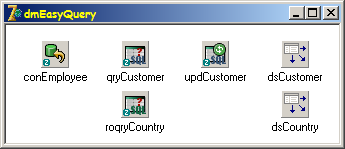
\includegraphics[width=0.7\textwidth]{ZeosTutorial/dmEasyQuery.png}
  \caption{dmEasyQuery}
  \label{fig:dmEasyQuery}
\end{figure}

TZConnection:
\begin{itemize}
  \item Database: Employee.fdb
  \item Name: conEmployee
  \item Password: "password"
  \item Protocol: firebird-1.5
  \item ReadOnly: False
  \item TransactionIsolationLevel: tiReadCommitted
  \item User: "username"
\end{itemize}

TZQuery:
\begin{itemize}
  \item Connection: conEmployee
  \item Name: qryCustomer
  \item RequestLive: True
  \item SQL: SELECT * FROM customer ORDER BY customer
  \item UpdateObject: updCustomer
\end{itemize}

Note: You have to create persistent TFields for all tablefields using the fieldeditor!

The OnAfterPost event of qryCustomer will be implemented like this:
\begin{verbatim}
procedure TdmEasyQuery.qryCustomerAfterPost(DataSet: TDataSet);
begin
  // Refresh of resultset to actualize (sort) data shown in DBGrid.
  qryCustomer.Refresh;
end;
\end{verbatim}

TZReadOnlyQuery
\begin{itemize}
  \item Connection: conEmployee
	\item Name: roqryCountry
	\item SQL: SELECT country FROM country ORDER BY 1
\end{itemize}

Note: You have to create persistent TFields for all tablefields using the fieldeditor!

TZUpdateSQL
\begin{itemize}
  \item DeleteSQL: created by UpdateSql editor
  \item InsertSQL: created by UpdateSql editor
  \item ModifySQL: created by UpdateSql editor
  \item Name: updCustomer
\end{itemize}

The delete-, insert- and modify-statements for the TZUpdateSQL object are created with the UpdateSQL editor, automatically.
The editor will be activated by double clicking on the TZUpdateSQL component.
As key field you have to select the field CUST\_NO. The fields ADDRESS\_LINE1, ADDRESS\_LINE2, CITY, STATE\_PROVINCE, COUNTRY und POSTAL\_CODE will selected as update fields in list "Update Fields".
Now the statements will be generated by clicking button "Generate SQL" (see firgures \ref{fig:dmEasyQuery_updCustomer_options} and \ref{fig:dmEasyQuery_updCustomer_sql}).
If you only have such easy queries you can save a lot of typing by using the UpdateSQL editor.
If it gets a little more complex you should create the needed statements "by hand".

\begin{figure}[htbp] 
  \centering
  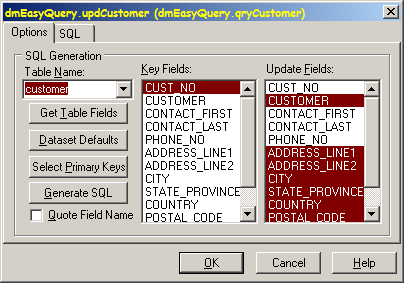
\includegraphics[width=0.7\textwidth]{ZeosTutorial/dmEasyQuery_updCustomer_options.png}
  \caption{options tab in UpdateSQL editor updCustomer}
  \label{fig:dmEasyQuery_updCustomer_options}
\end{figure}

\begin{figure}[htbp] 
  \centering
  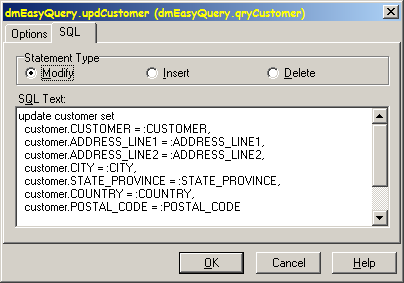
\includegraphics[width=0.7\textwidth]{ZeosTutorial/dmEasyQuery_updCustomer_sql.png}
  \caption{SQL tab in UpdateSQL editor updCustomer}
  \label{fig:dmEasyQuery_updCustomer_sql}
\end{figure}
	
TDataSource
\begin{itemize}
  \item DataSet: sqlCustomer
  \item Name: dsCustomer
\end{itemize}

TDataSource
\begin{itemize}
  \item DataSet: rosqlCountry
	\item Name: dsCountry
\end{itemize}

Now the created DataModule will be saved as dm\_EasyQuery.pas.

\subsection{Components for the form}
\begin{figure}[htbp] 
  \centering
  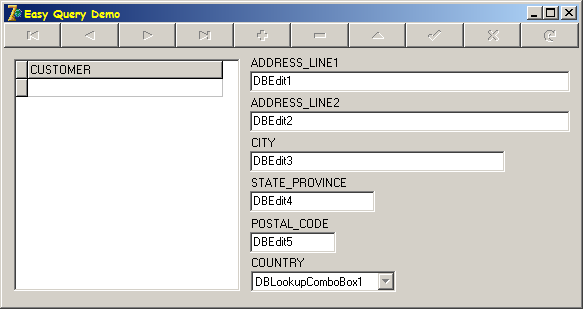
\includegraphics[width=0.7\textwidth]{ZeosTutorial/frmEasyQuery.png}
  \caption{EasyQuery main form}
  \label{fig:frmEasyQuery}
\end{figure}

The main form will have the following components and is initialized as follows:

Properties:
\begin{itemize}
  \item Caption: Easy Query Demo
  \item Name: frmEasyQuery
\end{itemize}

In the Unit's interface you have to add dm\_EasyQuery to the uses clause to get access to the database components.

The following events of the main form have to be implemented:

OnCreate:
When creating the form the connection to the database will be established.
After connecting to the database the queries will be opened:
\begin{verbatim}
procedure TForm1.FormCreate(Sender: TObject);
begin
  dmEasyQuery.conEmployee.Connect;
  dmEasyQuery.qryCustomer.Open;
  dmEasyQuery.roqryCountry.Open;
end;
\end{verbatim}

OnDestroy:
When closing the application (destroying the main form) the database connection will be cut.
All queries will be closed automatically before disconnecting.
\begin{verbatim}
procedure TForm1.FormDestroy(Sender: TObject);
begin
  dmEasyQuery.conEmployee.Disconnect;
end;
\end{verbatim}

TLabel
\begin{itemize}
  \item Caption: CUSTOMER
\end{itemize}

TDBGrid
\begin{itemize}
  \item DataSource: dmEasyQuery.dsCustomer
	\item Options.dgTabs: False
\end{itemize}

In column editor we will create a TColumn setting its property FieldName to "CUSTOMER".
After that the according column in DBGrid1 will be enlarged.

\begin{figure}[htbp] 
  \centering
  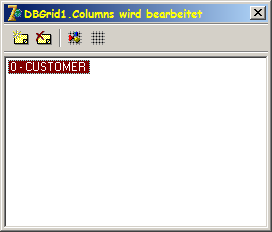
\includegraphics[width=0.7\textwidth]{ZeosTutorial/dbgrid1_columns.png}
  \caption{columns editor of DBGrid1}
  \label{fig:dbgrid1_columns}
\end{figure}

TDBEdit
\begin{itemize}
  \item (5x)
\end{itemize}

TLabel
\begin{itemize}
  \item (5x)
\end{itemize}

These objects will be created by using the columneditor of qryCustomer:
Select columns ADDRESS\_LINE1, ADDRESS\_LINE2, CITY, STATE\_PROVINCE and POSTAL\_CODE and drag and drop them onto then main form.
Align them and adapt them to the layout you see in the screenshot (figure \ref{fig:frmEasyQuery}).

TLabel
\begin{itemize}
  \item Caption: COUNTRY
\end{itemize}

TDBLookUpComboBox
\begin{itemize}
  \item DataField: COUNTRY
	\item DataSource: dmEasyQuery.dsCustomer
	\item KeyField: COUNTRY
	\item ListField: COUNTRY
	\item ListSource: dmEasyQuery.dsCountry
\end{itemize}

TDBNavigator
\begin{itemize}
  \item DataSource: dmEasyQuery.dsCustomer
\end{itemize}

Now the created form will be saved as frm\_EasyQuery.pas.

Note: The following project options have to be changed:

dmEasyQuery has to be placed on top of the creation order in list "Create automatically".
This ensures that all objects of frmEasyQuery may access the database objects.
frmEasyQuery is still the main form (see figure \ref{fig:EasyQuery_ProjectOptions}).
	
\begin{figure}[htbp] 
  \centering
  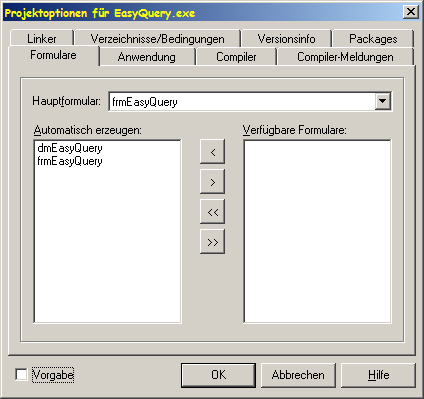
\includegraphics[width=0.7\textwidth]{ZeosTutorial/EasyQuery_ProjectOptions.png}
  \caption{EasyQuery project options}
  \label{fig:EasyQuery_ProjectOptions}
\end{figure}

\section{Additional Examples}
FishFact:
This is the most popular database demo for Delphi. It was migrated to use ZEOS components.

Transactions:
A sample application concerning "transactions with ZEOS". It uses a small self made test database.

StoredProc:
This is a sample applikation that shows how to use stored proecedures. The database is the Firebird
Employee sample database.

MasterDetail:
A small application that shows how master/detail connections (server and client sided) will be implemented.

EventDemo:
Also a Delphi database sample that was migrated from IBX to ZEOS.
It uses the component TIBEventAlerter.
This application needs the database Events (shipped with Delphi) that had to be migrated to dialect 3 to get this sample running.

\chapter{An Introduction To ZDBC API}
This document has been recovered from the original Zeoslib Foum Knoledge Base.

Zeos Database Connectivity Interface (or ZDBC for short) is a low-level API used by ZeosDBO to "hide" differences in native database client APIs and provide a uniform interface for high-level component layers. Originally, ZDBC was a port of JDBC 2.0 (Java Database Connectivity API) to Object Pascal. Since that time the API was slightly extended but the main ideas remain unchanged.

The main purpose of ZDBC is to be an intermediate layer in ZeosDBO. But it is also useful for application programming as it provides extremely light and fast access to SQL databases.

The best way to master ZDBC is to study the JDBC 2.0 specification http://java.sun.com/products/jdbc/jdbc20.pdf and then use analogy to convert JDBC abstractions and calls to ZDBC. To understand the role of ZDBC API in ZeosDBO architecture you may look at the Architecture Overview document http://www.zeoslib.net/modules.php?name=News\&file=article\&sid=23\&mode=\&order=0\&thold=0 For those who prefer a simpler introduction to ZDBC we propose a "hackers" guide as a starting point. 

\section{Pros and Cons of using ZDBC}
Before coding let's think why and when we should use ZDBC. Using ZDBC in applications has some clear benefits:
\begin{itemize}
  \item It's extremely fast and lightweight.
  \item It's database independent and supports many SQL servers. All supported SQL databases in ZeosDBO have correspondent ZDBC drivers.
  \item It does not require DB unit to be present. Some Personal Editions of Borland compilers do not include the DB unit with the TDataset implementation. This prevents the use of ZeosDBO components with these compilers.
\end{itemize}

There are also a few disadvantages which you need to consider carefully: 
\begin{itemize}
  \item It's not portable. You won’t be able to switch to other products without major changes in your applications (except Java and JDBC of course).
  \item It doesn't provide binding with data-aware visual controls. Implementation of such bindings manually can be a Herculean job.
  \item It doesn't contain all functionality of TDatasets such as client-side filtering, master-detail linking, sorting, etc.
\end{itemize}

So, from our point of view usage of ZDBC makes sense only in few special situations (of course you may have your personal opinion):
\begin{itemize}
  \item Your application is a console type application or does not allow users to edit relational data directly.
  \item Database access performance is very important.
  \item You don't care about porting your application to other database connectivity products.
\end{itemize}

\section{Establishing Connections}
In JDBC/ZDBC the entry point to the API is a special DriverManager object which serves as a factory for database connections. 

\begin{verbatim}
uses ZDbcIntfs...
...
var
  Connection: TZConnection;
...
Connection := DriverManager.GetConnection(<Connection URL>);
...
\end{verbatim}

Connection URL also comes from JDBC and has the following format:
\begin{verbatim}
zdbc:<protocol>://<host>[:<port>]/<database>[?<param1>[=<value1>]...]
\end{verbatim}

Protocol is essentially the name of the ZDBC driver you want to use. ZeosDBO version 6.1 has a number of protocols:
\begin{itemize}
  \item MySQL: mysql, mysql-3.20, mysql-3.23, mysql-4.0
	\item PostgreSQL: postgresql, postgresql-6.5, postgresql-7.2, postgresql-7.3
	\item Interbase: interbase, interbase-5, interbase-6
	\item Firebird: firebird, firebird-1.0, firebird-1.5
	\item Sybase: sybase
	\item MS SQL: mssql
	\item ADO: ado
\end{itemize}

Parameters in the connection URL specify different switches for the drivers.
There are several standard parameters for all drivers.
For other driver-specific parameters you need to refer to the ZeosDBO documentation. 
\begin{itemize}
  \item username – user name to connect to the database.
  \item password – user password to connect to the database.
  \item defaults \[yes \| no\] – calculate default values.
  \item update \[changed \| all\] – update only changed or all fields.
  \item where \[keyonly \| all\] – include where clause only key or all fields.
\end{itemize}

For example, to connect to MySQL 4.0 database with the compression protocol enabled you need to write:
\begin{verbatim}
uses ZDbcIntfs...;

...
var
  Connection: TZConnection;
...
Connection := DriverManager.GetConnection(
  'zdbc:mysql-4.0://localhost:3306/mydb?'
  + 'username=myuser;password=mypwd;compress=yes');
...
\end{verbatim}

If you want, you may specify the login and password separately: 

\begin{verbatim}
...
Connection := DriverManager.GetConnectionWithLogin(
  'zdbc:mysql-4.0://localhost:3306/mydb'
  + '?compress=yes', 'myuser', 'mypwd');
...
\end{verbatim}

Or you may specify parameters in a TStringList object:

\begin{verbatim}
...
var
  Connection: IZConnection;
  Params: TStrings;
...
Params := TStringList.Create;
Params.Values['username'] := 'myuser';
Params.Values['password'] := 'mypwd';
Params.Values['compress'] := 'yes';

Connection := DriverManager.GetConnectionWithParams(
  'zdbc:mysql-4.0://localhost:3306/mydb', Params);
\end{verbatim}

\section{Executing SQL statements}
We already know how to connect to our SQL database. But to do something useful you need to execute SQL statements. Let's look how to do that.

The simplest way to execute static SQL statements is the following:
\begin{verbatim}
var
  ...
  Statement: IZStatement;
  UpdatedRows: Integer;
...
Statement := Connection.CreateStatement;
UpdatedRows := Statement.ExecuteUpdate(
  'UPDATE MyTable SET MyField=''abc'' WHERE MyKey=123');
...
\end{verbatim}

Additionally to static SQL queries you can execute queries with parameters.
In some cases they may be more efficient because the parsing step is skipped.
But some SQL databases like MySQL or PostgreSQL don't support that feature and queries with parameters are emulated on the client side. 

\begin{verbatim}
var
  ...
  Statement: IZPreparedStatement;
  UpdatedRows: Integer;
...
Statement := Connection.PrepareStatement(
  'UPDATE MyTable SET MyField=? WHERE MyKey=?');

// Execute first update
Statement.SetString(1, 'abc');
Statement.SetInt(2, 123);
Statement.ExecutePrepared;

// Execute second update
Statement.SetString(1, 'xyz');
Statenent.SetInt(2, 789);
Statement.ExecutePrepared;
...
\end{verbatim}

If you execute several SQL queries one by one it makes sense to group them together in a single "batch update". 

\begin{verbatim}
...
Statement.AddBatch('UPDATE MyTable SET MyField=''abc'' WHERE MyKey=123');
Statement.AddBatch('UPDATE MyTable SET MyField=''xyz'' WHERE MyKey=789');
Statement.ExecuteBatch;
...
\end{verbatim}

Batch updates are also supported for prepared statements (statements with parameters): 

\begin{verbatim}
...
Statement := Connection.PrepareStatement(
  'UPDATE MyTable SET MyField=? WHERE MyKey=?');

// Execute first update
Statement.SetString(1, 'abc');
Statement.SetInt(2, 123);
Statement.AddBatchPrepared;

// Execute second update
Statement.SetString(1, 'xyz');
Statenent.SetInt(2, 789);
Statement.AddBatchPrepared;

Statement.ExecuteBatch;
...
\end{verbatim}

\section{Error Handling}
If any errors on the client or server side happens, ZDBC raises an EZSQLException exception.
This exception let you know not only the error message but also the error code from the server

\begin{verbatim}
try
  ...
  Statement.ExecuteUpdate(...);
   ...
catch
  on E: EZSQLException do
    WriteLn(Format('SQL Error: %d with Code: %d',
      [E.Message, E.ErrorCode]));
end;
\end{verbatim}

\section{Transaction Management}
Transaction management in ZDBC is controlled by the Connection object.
By default, Connection works in AutoCommit mode but it also provides you with all necessary methods to manage transactions manually.
Let's look how to execute SQL statements in a read-commited transaction:

\begin{verbatim}
...
Connection.SetAutoCommit(False);
Connection.SetTransactionIsolation(tiReadCommited);
...
try
  ...
  Statement.ExecuteUpdate(...);
  Statement.ExecuteUpdate(...);
  ...
  Statement.Commit;
except
  Statement.Rollback;
end;
...
\end{verbatim}

Please note that there is no out-of-transaction state.
Your connection object is always in-transaction so you don't need to start transactions manually.
Connection starts a transaction automatically when:
\begin{itemize}
  \item A connection is established
  \item AutoCommit or TransactIsolation level are changed
  \item Commit or Rollback are executed
\end{itemize}

JDBC considers this a safer approach.
You just need to be careful and complete transactions explicitly when you change AutoCommit or TransactionIsolation properties. 

\section{Retrieving data from SQL server}

Getting data from your SQL server may be the most interesting part of the story. Fortunately, it's not much more complicated than what we have seen so far. ZDBC API has two abstractions for queries: IZResultSet and IZResultSetMetadata. IZResultSet provides access to relational data retrieved as a result of executing a SELECT statement or a stored procedure. IZResultSetMetadata contains metadata for the query like: number of columns, column names and their types, etc.

The following example shows how to execute a SELECT statement and read its data:

\begin{verbatim}
var
...
  ResultSet: IZResultSet;
  Metadata: IZResultSetMetadata;
...
Statement := Connection.CreateStatement;
ResultSet := Statement.ExecuteQuery('SELECT * FROM MyTable');
Metadata := ResultSet.GetMetadata;

// Printing column headers
for I := 1 to Metadata.GetColumnCount do
  Write(Metadata.GetColumnName(I), ' ');
WriteLn;

// Printing query data
while ResultSet.Next do
begin
  for I := 1 to Metadata.GetColumnCount do
    Write(ResultSet.GetString(I), ' ');
  WriteLn;
end;
...
\end{verbatim}

SQL Queries can also contain parameters. Look at the next example to see how to use them:

\begin{verbatim}
...
var
...
  Statement: IZPreparedStatement;
  ResultSet: IZResultSet;
...
Statement := Connection.PrepareStatement(
  'SELECT * FROM MyTable WHERE MyKey=?');
Statement.SetInt(1, 123);
ResultSet := Statement.ExecuteQueryPrepared;
...
\end{verbatim}

The good news about ZDBC is that it allows you not only to read but also to write data.
You just need to set a ResultSetConcurrency mode for the Statement object.

\begin{verbatim}
...
Statement.SetResultSetConcurrency(rcUpdatable);
Statement.SetResultSetType(rtScrollInsensitive);
ResultSet := Statement.ExecuteQuery('SELECT * FROM MyTable');

...
// Insert a new row
ResultSet.MoveToInsertRow;
ResultSet.UpdateInt(1, 123);
ResultSet.UpdateString(2, 'abc');
ResultSet.InsertRow;
...
// Update row
ResultSet.UpdateString(2, 'xyz');
ResultSet.UpdateRow;
...
// Delete row
ResultSet.DeleteRow;
...
\end{verbatim}

\section{Advanced Topics}
This description of ZDBC API is not full.
ZDBC has many other features like Database Metadata, Blobs, Cached Updates, Stored Procedures, Sequence Generators, etc.
Unfortunately, due to size constraints, we couldn't discuss all of these topics in this article.
If you want to explore more of ZDBC you need to look at the JDBC specification and the source code of the ZDbcIntfs unit for more information.

(c) 2005 ZeosLib Team

\part{Zeos developer documentation}

\chapter{Getting Started with ZeosLib}
\section{Welcome to ZeosLib!}
Perhaps you began to read this document because you interested to join ZeosLib development team.
ZeosLib is an open-source freeware project which was founded by volunteers and still exists just because of non-paid contribution of many people who have a goal to help others.
You must be one of these altruists and we are glad to welcome you in ZeosLib!
We, old team members, will try to do the best we can to make you road to productive work in the project as simple and fast as possible.

\section{Study the Project}
Of cause, you must saw ZeosLib products already and have an idea what they do.
Probably you already know which area you’d like to contribute to the project.
In fact, the code you saw in ZeosLib releases is only a small part of the story.
To be sustainable the project has a lot of infrastructure around.
It includes project organization, tests and test databases, standards, procedures and practices.
To be productive you need to know all of those quite well.

To every new candidate we are saying the same things:
\begin{itemize}
  \item Send us your email to subscribe to the development mail list
	\item Study the project organization and structure
	\item Get source code from the project SVN repository
	\item Run your first tests
\end{itemize}

Just not long ago direct communication with experienced team members was the only source of information about the project.
It made quite high barrier to get started and see the “big picture”.
The situation is getting better now.
We understand the importance of normal project documentation and this document is one of our new “documentation initiative”.
Other documents are also available for you to read and can be requested from the project manager.

Although documents are good, the live conversation with people can not be replaced.
Team members have different ways to talk to each other, via personal mail, live chat sessions.
But the primary place of our conversations is the “ZeosLib development maillist”.

The development maillist is set up by SourceForge foundation and can be accessed at http://lists.sourceforge.net/lists/listinfo/zeoslib-devel.
The maillist is moderated.
It means you can’t subscribe or post there until you get an approval from the project manager.
So if you decided to join the development team, select one of your email addresses, where you’d like to receive the project related correspondence, and set it to the project manager.
When you subscribed, you’ll receive an email with notification. 

It is a good idea to learn about the project by reading development maillist archive.
You can do that at http://sourceforge.net/mailarchive/forum.php?forum=zeoslib-devel

The next your step will be to learn about the project organization and structure.
This topic is covered in a special document which is called “ZeosLib - Project Organization and Structure” [1].
It describes the project organization, main standards, project procedures and practices.
It also gives you an idea how ZeosLib products are structured in the project CVS repository.

\section{Access Project SVN Repository}
After you get initial information about the project internals you are ready to look how all that works.
To do that you need to obtain a copy of the project source code from SVN.

ZeosLib project is hosted on SourceForge and uses Subversion (SVN) to keep the code in one place and share it among project developers.
If you are not familiar with SVN yet it’s a good chance to learn about it.
SVN is widely used and information about it can be easily found in the Internet.
The good guide devoted to CVS is “Open Source Development with CVS” at http://cvsbook.red-bean.com/cvsbook.html.
SVN has a command line interface, so for those who like GUIs, there are many SVN frontends available.
The one which is used in our team is TortoiseSVN from https://tortoisesvn.net.

Once you installed CVS and learned basics how to use it you can get ZeosLib source code.
SourceForge has good documents which cover usage of SourceForge CVS.
To learn you can start from here: http://sourceforge.net/cvs/?group\_id=35994

ZeosLib has several products.
Each product is stored in CVS repository as an independent module.
There are several products/modules available:
\begin{itemize}
  \item zeosdbo\_rework – Zeos Database Objects (version 6.0 and up)
	\item zeosctrl\_rework – Zeos Controls (version 2.0 and up)
	\item zsql – Zeos SQL command line utility
	\item zde – Zeos Database Explorer (the old version)
	\item zdd – Zeos Database Designer (the old version)
\end{itemize}

ZeosLib active developers use SSH access to CVS repository to get the code and commit changes.
Until you get into all details of the project it’s safe for you and the project to work through anonymous PSERVER access in read-only mode.
When you prove you are ready to work you’ll be added to the project developers list on SourceForge and get an access through SSH.
Until that time you may use the following command:

\begin{verbatim}
> cvs –d:pserver:anonymous@cvs.sourceforge.net:/cvsroot/zeoslib co <module_name>
\end{verbatim}

For example to obtain the copy of ZeosDBO components run the following:

\begin{verbatim}
> cvs –d:pserver:anonymous@cvs.sourceforge.net/cvsroot/zeoslib co zeosdbo_rework
\end{verbatim}

\section{Run Tests}
Testing is one of the most important activities in the project.
You can meet tests almost everywhere: during development, nightly builds, release preparation and, of cause, support and bug fixing.
To support testing ZeosLib project has a special Test Framework and Build \& Test Environment (BTE).

To set up complete Build \& Test Environment quite few things you need to know.
Fortunately to run the tests and start playing with them you can use a shortcut. 

\begin{enumerate}
  \item
	  To get an idea why tests are so important and how they work you need to read “Fundamentals of Software Testing” document [2].
		It will give you some basic ideas about testing and explains about DUnit – unit testing framework for Object Pascal.
	\item
	  ZeosDBO code from CVS repository should be already in place. If you haven’t checked it out yet, it’s the right time to do that.
	\item
	  To run the tests you can use any supported database.
		To simplify your life we’ll explain who to use SQLite database in tests.
		SQLite is an extremely simple embedded SQL database engine and require minimal work to set it up.

    Download SQLite 2.8 from http://www.sqlite.org.
    You need to download sqlitedll-*.zip and sqlite-*.zip archives.
    Put sqlite.dll into your Windows/System directory and copy sqlite.exe into some place where you want to keep your test databases.

    Description of the tests and test databases is located in /database/test.properties file in your ZeosDBO directory.
    /database/test-template.properties contains an example.
    For you we recommend to create the file manually and put there the following lines (replace marked text with values appropriate for you):

\begin{verbatim}
[common]
common.configs=sqlite28

[sqlite28]
sqlite28.protocol=sqlite-2.8
sqlite28.host=localhost
sqlite28.database=<path to your sqlite dir>\zeoslib.db
sqlite28.user=
sqlite28.password=
sqlite28.rebuild=yes
sqlite28.createscripts=create_sqlite.sql,populate_any.sql
sqlite28.dropscripts=drop_sqlite.sql
\end{verbatim}

  \item
	  Run your compiler IDE, open ZeosDevel.bpg from /packages/$<$your compiler$>$/ directory. 
		Select View -$>$ Project Group to see the project group content.
		Select Project -$>$ Build All to compile the code.
		Add $<$path to zeosdbo$>$/packages/$<$your compiler$>$/build directory to Library Path in Tools -$>$ Environment Options -$>$ Library.

  \item
	  In the project group you can see several packages (.bpl) and executables (.exe).
		Packages contain the project source code; executables are required to run various tests to test the code.
		Select and run one-by-one the following tests:
		\begin{itemize}
		  \item ZTestCoreAll.exe – tests for ZCore.bpl package (Core classes and functions)
		  \item ZTestParseSqlAll.exe – tests for ZParseSql.bpl package (SQL lexical parsers and syntax analyzers)
		  \item ZTestDbcAll.exe – tests for ZDbc.bpl packages (Zeos DBC API)
		  \item ZTestComponentAll.exe – tests for ZComponent.bpl (ZeosDBO components)
		  \item ZTestBugReport.exe – tests for project bug reports
		\end{itemize}
		Leave ZTestPerformance test for now.
		You’ll learn how to set up and run performance tests later.
\end{enumerate}

If you did everything right you should get results like this:
\begin{verbatim}
DUnit / Testing
...........................................
Time: 0:00:04.717

OK: 34 tests
\end{verbatim}

If you get stacked at some point don’t worry.
Post a message to the development maillist and describe your problem.
Experienced team members will definitely help you to make it run!

\section{Continue the Work}
Congratulations, you have done the first step into ZeosLib project!
To become a fully-featured ZeosLib developer you need to know a little bit more.
Read the available documentation, set up and run the project Build \& Test Environment, learn the source code.
You need to study how to develop, test and support ZeosLib products.
Your first changes and tests you’ll commit into CVS through one of the experienced developers.
Your ultimate goal is to learn how to work in the project correctly to add valuable functionality and keep the code stable.
When you prove you can work according the project procedures, you’ll be added to the project developers list and get a right to commit changes into SVN yourself.

\section{Special Note for Hackers}
If you’d like join the project just to add your favorite DoAllWhatINeedInOneCall method, perhaps ZeosLib development group is not a good place for you.
Just think about the following: ZeosLib products are used by thousands people.
If everybody will stick into the code specific features he needs pretty soon the components will look like a garbage can. 

To delivery professional quality products ZeosLib development group follows strict Software Engineering Process.
Every new feature before going into development must be discussed how it should be implemented, what is the best place for it and, finally, does it need to be implemented at all.
Every piece of code must be developed according standards, accompanied with tests and supported on continues basis. 

If you have a great idea, try to subclass the components and put your lovely features there.
Professional software development is not a fun but a lot of routine, sometime unpleasant, work. Think about that…

\section{References}
\begin{enumerate}
  \item ZeosLib – Organization and Structure
  \item ZeosLib – Fundamentals of Software Testing
  \item ZeosLib – Build \& Test Environment
\end{enumerate}

\chapter{ZeosLib – Organization and Structure}

\section{General Overview}

ZeosLib is a freeware open-source project to provide professional quality database development tools to programming community. 

All work in the project is done by volunteers, who joined the project on permanent base, and contributors, who kindly present their code and documents.
We appreciate any help and thank everybody who gives it to us.
Additionally we started “Cooperating Projects” program.
It is intended to individuals and companies who prefer to stay out of the project but develop products in relation to our work.
Under “Cooperating Project” you can see various freeware open-source extensions to our components as well as other components or tools which are based on ZeosLib or integrated with it.

Our products are free of charge, even for commercial project, and distributed under Lesser GNU public license.
Users are free to use our products, modify the source code and include them into own applications.
The only things we are trying to restrict are changing our copyrights and reselling the components and tools in any form except in working end-user applications.  

Although all our products are free development team keeps a right to provide valuable commercial services around the project.
It may include hot user-support, documentation, consulting – anything which may increase quality of the products, help our users and support team members in their hard work.

\section{Project Scope}
All products developed in the project are concentrated around SQL databases.
Our project consists with various component libraries oriented for database application developers and ready to use tools for database administrators and end-users.
Our core product is “Zeos Database Objects” – a set of native database components written in Object-Pascal programming language.

At the moment the list of ZeosLib products is the following:
\begin{itemize}
  \item Zeos Database Objects – a library of native database connectivity components.
  \item Zeos Controls – a library of visual controls to support database application development.
	\item Zeos SQL – a command-line tool to execute SQL, similar to mysql, psql, isql utilities, but with support for all ZeosLib-compatible SQL servers.
	\item Zeos Database Explorer – a GUI utility to execute SQL statements, view database metadata, and edit database tables and large objects (BLOBs).
	\item
	  Zeos Database Designer – a GUI database schema designer.
		The big advantage of this tool that it supports generation of portable SQL which will work with ZeosDBO across all supported databases.
\end{itemize}

All the products within ZeosLib project are developed in Borland Delphi.
It means they are written in Object Pascal programming language and use VCL/CLX component model.
That fact limits the scope of our development components by development tools which support Object Pascal and VCL/CLX.
The list of compatible compilers includes Borland compilers - Delphi, C++ Builder and Kylix, and free open-source alternative compilers such as Free Pascal and Lazarus.
Our development tools are more generic and not bind to any compiler. They can be used by anybody who is working with relational databases.

The one significant advantage of our project is a wide coverage.
We are trying to support a large number of SQL databases, their versions and a long list of compilers.

Starting from the version ZeosDBO 6.5 the list of supported SQL servers is the following:
\begin{itemize}
  \item MySQL 3.20, 3.23, 4.0, 4.1
	\item PostgreSQL 6.5, 7.0, 7.2, 7.3, 7.4
	\item Interbase 5.0 – 7.0
	\item Firebird 1.0, 1.5
	\item MS SQL 6.5, 7.0, 2000
	\item Sybase ASE 12.0, 12.5
	\item SQLite 2.8
	\item Oracle 9i
\end{itemize}

The supported compilers are:
\begin{itemize}
  \item Delphi 5, 6, 7 (version 8 is coming soon)
	\item C++ Builder 5, 6 (version X is coming soon)
	\item Kylix 2, 3
	\item Free Pascal Lazarus 0.93 (coming soon)
\end{itemize}

\section{Organization}
ZeosLib is a technically complex project.
Without proper organization it’s impossible to develop a respectable and stable product within the selected scope.
On other hand the project uses volunteering non-paid work and it’s hard to ask people who have no obligation to follow strict rules and procedures.
Keeping that in mind we are trying to concentrate only on vital aspects of the work, keeping our process as light as possible to avoid unnecessary overhead and encourage personal interest. 

ZeosLib project is developed and maintained by ZeosLib development team.
The team consists with 3 groups: “Development Group”, “Quality Assurance Group” and “Documentation and Support Group”:

\begin{description}
  \item [Development Group] is responsible to define product requirements, develop products and associated tests, port products to supported platforms and compilers, fix found bugs.
	\item [Quality Assurance Group (QA Group)] is responsible for maintaining project infrastructure, prerelease testing, releases, processing bug reports and replication of bugs in a form of “test cases”.
	\item [Documentation and Support Group] is responsible for writing product documentation, tutorials and examples, maintaining project web-site and national mirrors, preparation of FAQs and other user related documentation, users support through web-forums, advertising of the project in Internet.
\end{description}

The project has a “Project Manager”. In his responsibilities are administration tasks such as:
\begin{itemize}
  \item Stuffing of the project
	\item Planning of product releases
	\item Enforcement of project procedures and practices
\end{itemize}

Except a “Project Manager” there is a “CoManager” which performs duties of the “Project Manager” in his absence.

Each of the three groups in the project has a “Group Coordinator”.
“Group Coordinator” is responsible for definition of the direction of the group’s work and task allocation.

Because the project has a very limited number of people we do not strictly separate them by groups at the moment.
The “Group” now is mostly logical direction or type of work, but not an organization entity.
Every team member may select where he wants to participate and work in several groups at the same time.
The good example of such organization is the work of project developers.
When they are doing development they are acting within “Development Group”.
When they do testing as a part of release preparation their work is coordinated by “QA Group”.

Positions of “Project Manager”, “Project CoManager” and “Group Coordinators” are elective.
Any project member may ask for reelection for any position at any time.
If majority of team members are agree with that, the position holder will be dismissed and replaced by another person.

One of the fundamental rules in the project is a separation by “areas of responsibility”.
Each logical area in the project has an assigned “responsible person”.
The “responsible person” has a big freedom in his “area”.
He can select the most preferable way to perform his work.
He may initiate changes and do improvements within the scope.
Nobody else can do anything in the his area until he gets an approval from the “responsible person”.
The “responsible person” takes responsibilities for his area and must fix problems when they are found. 

The “areas of responsibility” allow us to prevent conflicts of interests and stimulate motivation in the end results.
Although there are few restrictions are applied to keep the project under control:
\begin{itemize}
  \item All the work must be done in accordance with project standards, procedures and practices.
	\item If some change lays out of scope for the current release, defined by Group Coordinator, or if it affects other areas of the project or project end users, it must be coordinated and approved by the Group Coordinator prior to implementation.
\end{itemize}

\section{Structure}
ZeosLib is a multi-product project.
It is hosted on SourceForge and the project structure is coming from those points.
All the project code, scripts and documents are controlled by CVS version control system, located on SourceForge servers.
Each product is represented as a high level module in the CVS repository:
\begin{verbatim}
/zeosdbo
/zde
/zsql
/zdd
/zeosctrl
\end{verbatim}

Each module contains all related source code, documentation, packages and scripts.
At the moment the typical one project (product) structure is the following:

\begin{description}
  \item [/build] scripts for Build \& Test Environment
  \item [/database] database SQL scripts and settings required for tests
  \item [/doc] project and user documentation
    \begin{description}
      \item [/develop] development documentation (is not included into releases)
      \item [/user] user documentation (included into releases)
      \item [/release] various release notes (Changes, ReadMe, Install) included into the root dir in release package.
		\end{description}
	\item [/example] sample projects which present how to use the product
  \item [/lib] various external libraries required to run the product
  \item [/package] packages (user and development) required to compile the product
    \begin{description}
		  \item [/$<$compiler 1$>$]
      \item [...]
      \item [/$<$compiler N$>$]
		\end{description}
	\item [/src] the project source code
	\item [/test] the project testing code
\end{description}

The infrastructure of the project is called “Build \& Test Environment” (BTE for short).
BTE turns a pile of code into a professional product.
All build scripts, database scripts, testing framework are parts of the BTE.

The main functions of the “Build \& Test Environment” are the following:
\begin{itemize}
  \item Provide to developers and QA group members a comprehensive testing framework to test the project
	\item Provide a consistent testing platform for continues integration, nightly build and pre-release tests to cover all supported compilers and SQL servers
	\item Compile the project code and generate the product documentation
	\item Prepare release distribution packages
\end{itemize}

At the moment BTE consists with few ANT scripts http://jakarta.apache.org/ant to perform the project goals: Clean, Compile, Test, Release, ReleaseDoc.
Unfortunately ANT is a very generic and low-level tool and does not provide a consistent platform for Project Management tasks and hard to reuse across multiple projects.
For the purpose to enhance and improve BTE we are looking at other more high-level project management tools such as Maven http://maven.apache.org .

\section{Standards, Procedures and Practices}
As it was said in the “Organization” chapter we are trying to keep the project as simple as possible and avoid unnecessary overhead introduced by formal process.
There are only few things which we think are vital for the project success.

The output of our work is the source code and documentation.
It is a matter of professionalism to keep it consistent and nice looking whoever did it.
At the moment we are trying to maintain two standards:
\begin{itemize}
  \item Standard for Source Code
	\item Standard for Written Documentation
\end{itemize}

There are few established procedures and practices in the project:
\begin{itemize}
  \item Development Procedure
	\item Release Procedure
	\item Bug Reporting Procedure
\end{itemize}

Development Procedure ensures the consistency and maintainability of the project.
It defines the next steps:
\begin{enumerate}
  \item Coordinate and get an approval to implement a feature from the Development Group Coordinator prior to start it.
	\item Follow Coding Standard when writing a code
	\item Implement tests together with the code to cover the most important functionality
	\item Port the code to all supported compilers (or coordinate with others to do that)
	\item Test the code with all supported compilers and SQL servers (or coordinate with others to do that)
	\item Support the code and fix bugs after product is released
\end{enumerate}

Release Procedure is important to archive the stability of the product releases.
\begin{itemize}
  \item
	  On Alpha stage of the product development any changes are allowed.
		On that stage all massive changes in the code must be completed.
	\item
	  On Beta stage only minor changes in the product functionality are allowed.
		Any new feature on that must be approved by Development Coordinator (QA Coordinator and Project Manager in line).
	\item
	  On Gamma stage any changes in the functionality are prohibited.
		Only bug fixes and tests can be done.
\end{itemize}

The Release Procedure should be accomplished for every major or minor release and includes the following steps:
\begin{enumerate}
  \item Prepare a release plan by Project Manager
	\item Announce the beginning of release preparation stage by QA Coordinator
	\item Stop all development activities
	\item Start comprehensive testing under all supported compilers and SQL servers
	\item When bugs are found, report them to responsible developers, fix and repeat all the testing from the beginning
	\item Update Change Notes, Release Notes and prepare a Release Announce
	\item Build a release distribution package
	\item Upload the release package to SourceForge “File Release Manager”
	\item Notify subscribed users on SourceForge
	\item Add a link to “Downloads” page on the project web site and national mirrors.
	\item Submit an Announce Page on the site and national mirrors
\end{enumerate}

The correct bug reporting procedure is absolutely critical to improve the quality of the products.
It defines steps to fix bugs, to notify the reported user about the change and update the test harness to ensure the bug will never happen again.
Unfortunately in freeware project it’s hard to maintain good test coverage.
The Bug Report procedure allows improving the test coverage and increasing the stability of the products afterwards, when the code is written and released.
It relieves developers because writing tests is partially moved to responsibilities of QA group.

Bug Reporting Procedure consists with the following steps:
\begin{enumerate}
  \item User submits a bug report on SourceForge bug tracker.
	\item
	  Elaborate information about the bug and close the bug it is has no sense.
		Notify the user about the action takes and explain why it was done (Performed by QA Group).
	\item Implement a Bug Report Test Case which replicates the problem (Performed by QA Group).
	\item Switch the bug to the responsible developer.
	\item Fix the bug (Performed by Responsible Developer)
	\item Close the bug report and notify the user about the change done (if it possible) and mention when it will be officially released (Performed by Responsible Developer).
\end{enumerate}

\chapter{ZeosLib Build \& Test Environment}

Majority of projects have some way to automate repetitive tasks such as compiling source code or building release artifacts.
It can be done with help of old Unix makefiles, XML ant scripts or using ultra-modern project management tools.
ZeosLib project is not an exception.

\section{General Overview}
Majority of projects have some way to automate repetitive tasks such as compiling source code or building release artifacts.
It can be done with help of old Unix makefiles, XML ant scripts or using ultra-modern project management tools.
ZeosLib project is not an exception.

ZeosLib project has a notion of Build \& Test Environment (BTE).
Under BTE we understand a set of tools, required to work in the project and automation scripts to perform common project tasks.

Tools, required for ZeosLib project tasks:
\begin{itemize}
  \item Java Standard Development Kit (JSDK)
	\item ANT make tool
	\item Maven project management tool
	\item Cygwin Unix emulation package for Windows
\end{itemize}

Tools, required for ZeosLib documentation:
\begin{itemize}
  \item FOP formatting objects processor
	\item Html Help compiler
	\item DoxyGen source doc generation tool
	\item XMLSpy XML editor
	\item Together UML modeling tool
\end{itemize}

The common tasks automated by Build \& Test Environment are:
\begin{itemize}
  \item Cleaning up generated files
	\item Compile source code using specified compilers
	\item Run tests for specified compilers and databases
	\item Generate project documentation
	\item Build project release distribution
\end{itemize}

Before start detail description of BTE we must say one more thing.
The implementation of Build \& Test Environment at the moment of writing this document (august 2004) is far from ideal.
BTE relies on custom ANT scripts.
These scripts do their work, but can not be easily reused across multiple projects.
To improve consistency and reusability of BTE we made a decision to replace ANT with Maven project management tool.
Maven in opposite to low-level make tools like ANT proposes a new level of abstraction.
It’s called Project Object Model (POM).
All tasks in Maven are implemented in highly generic fashion and take information about the project structure from POM.
POM separates project details from task scripts and greatly increases reusability of BTE. 

\section{Required Tools}

There is a set of tools required to work with ZeosLib BTE.
Some of them are required to run scripts and execute common tasks; others are needed to work on project documentation.

\subsection{Java Standard Development Kit}
Java Standard Development Kit is a mandatory component which must be installed on computer where BTE runs.
Java implements a truly portable language and virtual machine to execute programs on different platforms.
That is very important for us, because one of the main requirements is to run BTE on all supported platforms.
At the moment these platforms are Windows and Linux.

Installation instructions:
\begin{enumerate}
  \item Go to http://java.sun.com and download the latest J2SE 1.4 SDK
	\item Install Java SDK on your computer
	\item
	  Add environment variable JAVA\_HOME and set it equal to the path where JSDK is installed.
		For example: JAVA\_HOME=C:\\Program Files\\Java\\j2sdk\_1.4.2\_05
	\item Add to the system PATH environment variable a path to Java like \%JAVA\_HOME\textbackslash\textbackslash bin
	\item Check installation of Java executing the next command in command prompt:
	  \begin{verbatim}
C:\\>java -version
java version "1.4.2_05"
Java(TM) 2 Runtime Environment, Standard Edition (build 1.4.2_05-b04)
Java HotSpot(TM) Client VM (build 1.4.2_05-b04, mixed mode)
    \end{verbatim}
\end{enumerate}

\subsection{Cygwin}
Cygwin is another mandatory component of ZeosLib BTE.
It is a toolkit developed under RedHat umbrella in order to port Unix environment to Windows platform.
Cygwin includes a lot of famous Unix utilities such as ssh, cvs, make, bash, ftpd, etc.
Cygwin brings Windows environment as close to Unix as possible and gives us as an opportunity to use the same set of tools on both platforms. 

Installation instructions:
\begin{enumerate}
  \item Go to http://www.cygwin.org and click “Download Now”
	\item In Setup utility set Default Text Type to “DOS”, choose the mirror you want to use and select components to install.
    \begin{figure}[htbp] 
      \centering
      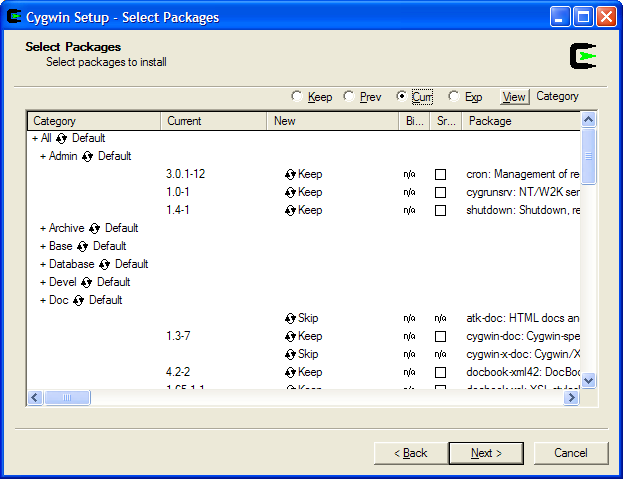
\includegraphics[width=0.7\textwidth]{BTE/CygwinSetup.png}
      \caption{dmEasyQuery}
      \label{fig:CygwinSetup}
    \end{figure}
		Please, make sure you selected to next components:
		\begin{itemize}
		  \item open-ssh (ssh tools to connect to ZeosLib cvs through ssh protocol)
			\item cvs (concurrent version control system)
			\item postresql (Windows port of PostgreSQL database)
			\item docbook-xml (DocBook XML DTD)
			\item docbook-xsl (DocBook XML StyleSheets to generate various output)
			\item xmlto (Simple script for common DocBook generation tasks)
			\item links (Text Web browser to generate Plain Text output for DocBook)
			\item lynx (Text Web browser to generate Plain Text output for DocBook)
		\end{itemize}
	\item 
	  Add to the system PATH environment variable a path to Cygwin bin directory.
		For example: C:\textbackslash Cygwin\textbackslash bin
	\item Add environment variable CVS\_RSH=ssh
	\item Check installation of Cygwin running in command line the following commands:
	  \begin{verbatim}
==============================================
C:\>bash
bash-2.05b$
bash-2.05b$ ssh -V
OpenSSH_3.7.1p2, SSH protocols 1.5/2.0, OpenSSL 0.9.7c 30 Sep 2003
bash-2.05b$
bash-2.05b$ cvs -v

Concurrent Versions System (CVS) 1.11.6 (client/server)

Copyright (c) 1989-2003 Brian Berliner, david d `zoo' zuhn,
                        Jeff Polk, and other authors

CVS may be copied only under the terms of the GNU General Public License,
a copy of which can be found with the CVS distribution kit.

Specify the --help option for further information about CVS
bash-2.05b$
bash-2.05b$ xmlto --help
usage: xmlto [OPTION]... FORMAT XML
OPTIONs are:
  -v              verbose output (-vv for very verbose)
  -x stylesheet   use the specified stylesheet instead of choosing one
  -m fragment     use the XSL fragment to customize the stylesheet
  -o directory    put output in the specified directory instead of
                  the current working directory
  -p postprocopts pass option to postprocessor
  --extensions    turn on stylesheet extensions for this tool chain
  --searchpath    colon-separated list of fallback directories
  --skip-validation
                  do not attempt to validate the input before processing

Available FORMATs depend on the type of the XML file (which is
determined automatically).
FIND: Invalid switch
bash-2.05b$
bash-2.05b$ lynx -version
Lynx Version 2.8.4rel.1 (17 Jul 2001)
libwww-FM 2.14, SSL-MM 1.4.1, OpenSSL 0.9.7b
Built on cygwin Aug 11 2003 22:59:49

Copyrights held by the University of Kansas, CERN, and other contributors.
Distributed under the GNU General Public License.
See http://lynx.browser.org/ and the online help for more information.
See http://www.moxienet.com/lynx/ for information about SSL for Lynx.
See http://www.openssl.org/ for information about OpenSSL.

bash-2.05b$$ % the second $ was added to have correct syntax highlighting in TexnicCenter.
===========================================================
    \end{verbatim}
\end{enumerate}

\subsection{ANT}

ANT is a famous Java and XML based make tool.
It is used to interpret current ZeosLib automation scripts.
ANT is much more sophisticated then old Unix make.
It proposes a lot of standard tasks in truly platform independent manner.

Installation instructions:
\begin{enumerate}
  \item Go to http://ant.apache.org and download the latest stable binary distribution (1.6.2 at the moment)
	\item Unzip ANT to some directory on your hard drive
	\item
	  Add ANT\_HOME environment variable and set it equal to the path to ANT directory.
		For example: ANT\_HOME=C:\textbackslash Program Files\textbackslash ant\_1.6.2
	\item Add to the system PATH environment variable a path to ANT tool as \%ANT\_HOME\%\textbackslash bin
	\item Check the installation running in the command prompt the following command:
	  \begin{verbatim}
C:\>ant -version
Apache Ant version 1.6.2 compiled on July 16 2004
    \end{verbatim}
\end{enumerate}

\subsection{Maven}
Maven is another Java and XML based build tool.
In opposite to ANT it proposes a new level of abstraction for common project tasks.
Maven introduces Project Object Model (POM) which separates project specific details from the generic project tasks.
That fact greatly improves reusability of the common tasks across multiple projects.
Inheritance of POM makes possible to enforce project rules across all subprojects.

At the moment Maven is not used in BTE.
We added these instructions to prepare ZeosLib team members to simplify their switch to this tool from ANT.

Installation instructions:
\begin{enumerate}
  \item Go to http://maven.apache.org and download the latest stable binary distribution
	\item Install Maven into some directory on your hard drive
	\item
	  Add MAVEN\_HOME environment variable and set it equal to the path to Maven directory.
		For example: MAVEN\_HOME=C:\textbackslash Program Files\textbackslash maven\_1.0
	\item Add to the system PATH environment variable a path to Maven tool as \%MAVEN\_HOME\%\textbackslash bin
	\item Check the installation running in the command prompt the following command:
	  \begin{verbatim}
C:\>maven -v
|  \/  |__ _Apache__ ___
| |\/| / _` \ V / -_) ' \  ~ intelligent projects ~
|_|  |_\__,_|\_/\___|_||_|  v. 1.0
    \end{verbatim}
\end{enumerate}

\subsection{FOP}

Formatting Objects Processor (FOP) is required to generate PDF output from DocBook files.

Installation instructions:
\begin{enumerate}
  \item Go to http://xml.apache.org/fop and download the latest binary distribution (0.20.5 at the moment)
	\item Unzip it to some directory on your hard drive
	\item 
	  Add FOP\_HOME environment variable and set it equal to the path to FOP directory.
		For example: FP\_HOME=C:\textbackslash Program Files\textbackslash fop\_.0.20.5
	\item Add to the system PATH environment variable a path to FOP as \%FOP\_HOME\%
	\item
	  Check the installation running in the command prompt the following command:
		\begin{verbatim}
===========================================
C:\>fop

USAGE
Fop [options] [-fo|-xml] infile [-xsl file] [-awt|-pdf|-mif|-pcl|-ps|-txt|-at|-p
rint] <outfile>
 [OPTIONS]
  -d             debug mode
  -x             dump configuration settings
  -q             quiet mode
  -c cfg.xml     use additional configuration file cfg.xml
  -l lang        the language to use for user information
  -s             (-at output) omit tree below block areas
  -txt.encoding  (-txt output encoding use the encoding for the output file.
                 The encoding must be a valid java encoding.
…..
============================================
    \end{verbatim}
\end{enumerate}

\subsection{HTML Help}
HTML Help compiler is required to generate HTML Help files from the project documentation.

Installation instructions:
\begin{enumerate}
  \item
	  Go to http://www.microsoft.com/downloads.
		Then make a search by “Html Help” keyword, find “HTML Help Workshop and Documentation” and download htmlhelp.exe file.
  \item Install HtmlHelp on your computer.
	\item To check the installation try to run HTML Help Workshop from Start -> Programs
\end{enumerate}

\subsection{DoxyGen}

DoxyGen is a tool to generate documentation directly from source code.
At the moment of writing this document DoxyGen was defined as the most preferable choice for sourcedoc generation, but we haven’t committed it yet.

You may download DoxyGen tools from the following locations:
\begin{enumerate}
  \item http://www.sourceforge.net/projects/doxygen
	\item http://www.sourceforge.net/projects/pasdoc
\end{enumerate}

\subsection{XMLSpy}

DocBook is a widely used XML format for documentation purposes.
It allows generating from single source documents in various formats: HTML, PDF, Html Help, Plain Text and others.
To work with DocBook you can use a simple text editor such as Notepad and then run xmlto command from Cygwin package to generate documents.
Although, for some people, who get used to WYSIWYG style tools, that approach can be uncomfortable.
To make the life simpler there are many existing commercial and free tools available in the Internet. 

The one of the best tools to work with DocBook documents is XMLSpy.
It is a commercial tool developed by Altova.
XMLSpy provides a very comfortable XML editor and generates an HTML output from edited XML document on-fly.
A trial version of XMLSpy can be downloaded from Altova website at http://www.xmlspy.com

There are couple pictures to give you some ideas about XMLSpy.

\begin{figure}[htbp] 
  \centering
  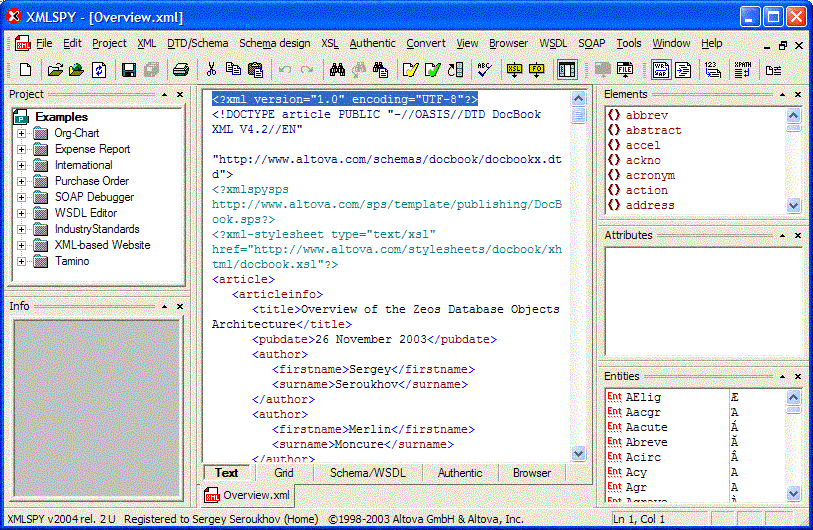
\includegraphics[width=1.0\textwidth]{BTE/XmlSpy1.png}
  \caption{XMLSpy 1}
  \label{fig:XmlSpy1}
\end{figure}

\begin{figure}[htbp] 
  \centering
  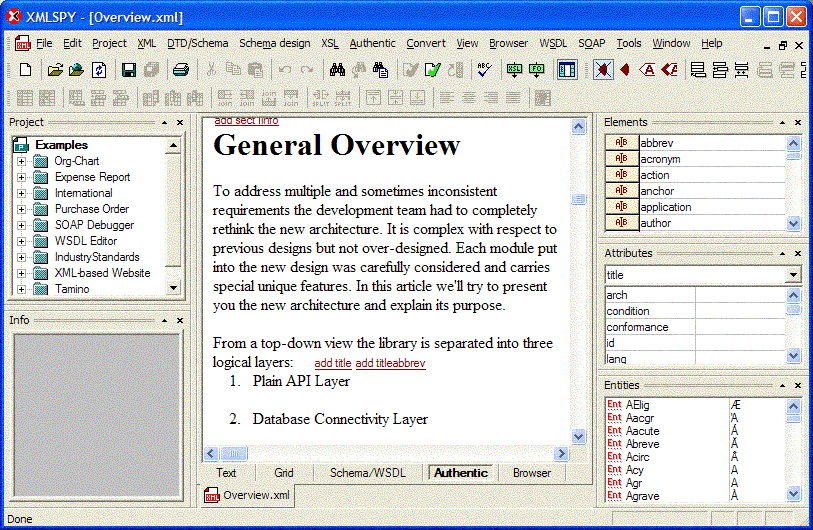
\includegraphics[width=1.0\textwidth]{BTE/XmlSpy2.png}
  \caption{XMLSpy 2}
  \label{fig:XmlSpy2}
\end{figure}
				
\subsection{Together}

Together is one of the world best UML modeling tools developed by Borland Corp.
It is very good news that Borland released a free Community Edition version of Together which we’d like to use for documentation tasks in ZeosLib project.
Additionally to standard UML diagrams Together proposes ER-diagrams which are very useful to design relation databases.
The limitation of Together Community Edition is that it does not include two important UML activity diagrams – Sequence and Collaboration.
But we think that Package and Class diagrams will be enough for our simple documentation tasks.

Installation instructions:
\begin{enumerate}
  \item Go to Borland Together website at http://www.borland.com/together
	\item Request a key for Together Community Edition. When you receive the key via email, copy it to your home catalog
	\item Download and install Together Community Edition
\end{enumerate}

There are few pictures to present you capabilities of Together.

\begin{figure}[htbp] 
  \centering
  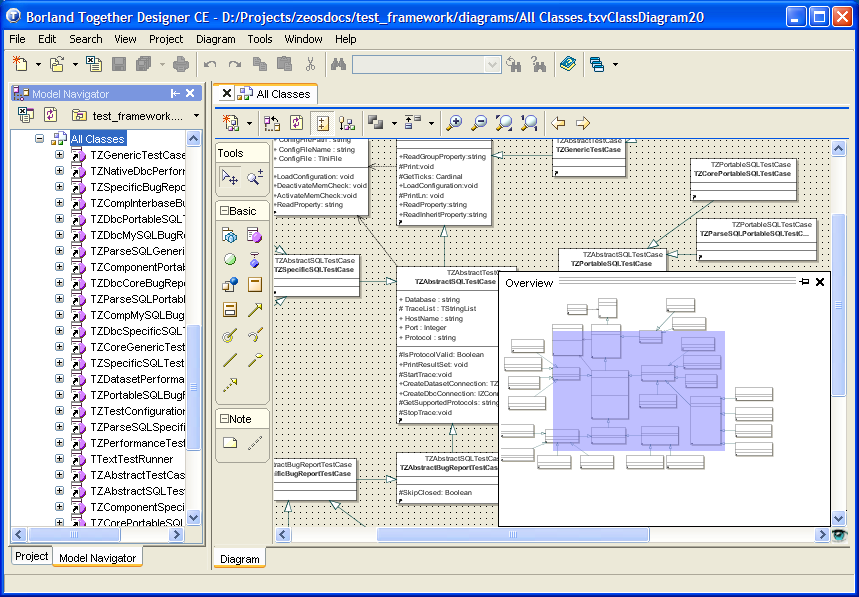
\includegraphics[width=1.0\textwidth]{BTE/Together1.png}
  \caption{Togeter 1}
  \label{fig:Together1}
\end{figure}

\begin{figure}[htbp] 
  \centering
  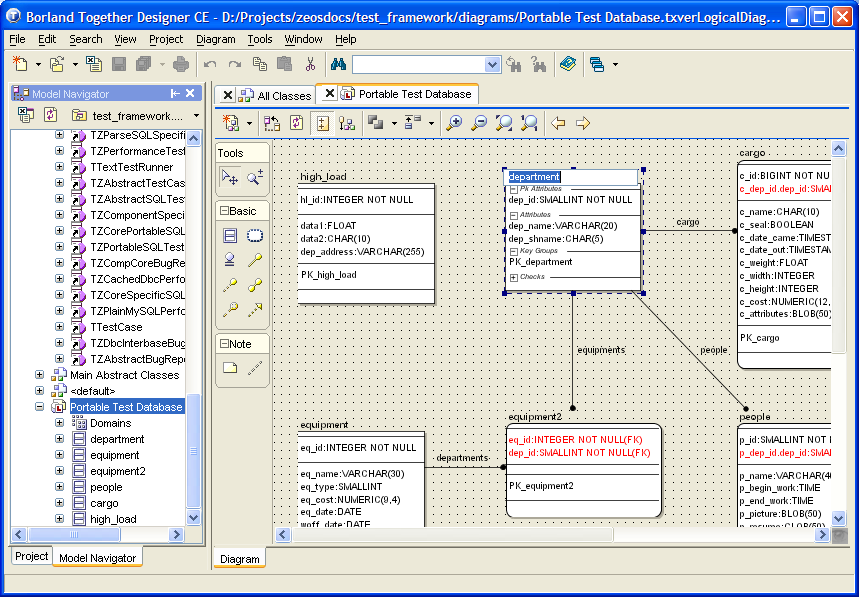
\includegraphics[width=1.0\textwidth]{BTE/Together2.png}
  \caption{Together 2}
  \label{fig:Together2}
\end{figure}

\section{Directories structure}
ZeosLib project directory structure is another important thing.
Because ZeosLib is a multi product project we are trying to reuse the same directory structure across all subprojects to ensure project consistency.
When BTE will be switched to Maven, the directory structure can be changed, but we do not expect major changes in that area.

Every ZeosLib subproject is stored in CVS repository as a separate module.
When you do checkout you may want to put all subprojects into one directory.
Moreover you may want to work with different branches of each subproject.
To do that the recommended way is to rename subproject top catalog.
For example:
\begin{verbatim}
> cvs –d:ext:developer@cvs.sourceforge.net:/cvsroot/zeoslib co –r v6_0_final zeosdbo_rework
> rename zeosdbo_rework zeosdbo_6_0
> cvs –d:ext:developer@cvs.sourceforge.net:/cvsroot/zeoslib co –r v6_1_final zeosdbo_rework
> rename zeosdbo_rework zeosdbo_6_1
> cvs –d:ext:developer@cvs.sourceforge.net:/cvsroot/zeoslib co zeosdbo_rework
> rename zeosdbo_rework zeosdbo_6_5
\end{verbatim}

The complete top-level directory structure could be the following:
\begin{verbatim}
C:\Projects\zeoslib
+ zde
+ zeosdbo_5_5
+ zeosdbo_6_0
+ zeosdbo_6_1
+ zeosdbo_6_5
+ zeosctrl_2_0
+ zeosctrl_2_1
+ zsql
\end{verbatim}

As we said before, for each subproject we are trying to follow the same directory structure:
\begin{verbatim}
zeoslib_project
+ build
+ database
+ doc
  + project
  + release
  + user
+ examples
  + <example 1>
  + <example 2>
  + <example 3>
+ lib
+ packages
  + <compiler 1>
    + build
  + <compiler 2>
    + build
+ releases
+ src
  + <package 1>
  + <package 2>
  + Zeos.inc
+ test
  + <package 1>
  + <package 2>
\end{verbatim}

The detail description of the project catalogs:
\begin{enumerate}
  \item Build – keeps BTE build scripts and build configuration in build.properties file.
	\item Database – contains SQL scripts to create and drop test database objects (portable and specific) and test configuration in test.properties file.
	\item Doc – contains all documentation in XML DocBook format.
	  \begin{itemize}
		  \item project – Project related documentation. It is not included into release distribution and services for project internal purposes
			\item release – Release notes such as README, INSTALL, KNOWN\_BUGS. These files are generated in Plain Text format and included into the root catalog of the release distribution
			\item user – A user documentation. It is included into release distribution into doc catalog.
		\end{itemize}
  \item
    Each documentation catalog contains DocBook files named as \textless document \textgreater .xml.
    Additionally it has images subcatalog to keep images related to the documents.
    The conversion to name image files is \textless document\textgreater\textless num\textgreater.\textless ext\textgreater. For example:
    \begin{verbatim}
doc
  + project
    + images
      + Overview1.jpg
      + Overview2.gif
   + Overview.xml
    \end{verbatim}		
  \item
	  Examples – various user examples and tutorials.
		Each subdirectory has an independent example project with all required source and data files.
	\item
	  Lib – external libraries required to compile or run the product.
		For example: ZeosDBO project has there supported libmysql and libpq dlls to connect to different versions of MySQL and PostgreSQL servers.
  \item
	  Packages – compilation packages for all supported compilers.
		Each subdirectory is named according compiler name and version (fpc10, cbuilder5, delphi7, etc).
		Build subdirectory is set to keep all binaries (.dcu, .obj, .exe…) generated during the compilation project. 
		
		If specific compiler supports project groups, the compiler package directory should contain two project groups: 
		\textless Project\textgreater.bpg with release packages only and \textless Project\textgreater Devel.bpg with all packages and test applications available in the project.
		These project groups greatly simplify installation and development tasks when they are done from compiler IDE.

	  The example taken from ZeosDBO project:
    \begin{verbatim}
+ packages
   + fpc10
     + build
   + cbuilder5
     + build
     + ZeosDbo.bpg
     + ZeosDboDevel.bpg
     …
   + delphi7
     + build
     + ZeosDbo.bpg
     + ZeosDboDevel.bpg
      …
    \end{verbatim}
  \item
		Releases – keeps release and documentation distribution packages.
		This directory is created automatically when release tasks are executed.
	\item
	  Src – a directory to keep the project production code.
		If project is complex, it may be required to split the code into separate packages; each package is own directory.
		Zeos.inc file has all compilation directives for the project.
	\item
	  Test – a directory similar to Src, but it keeps project tests which are not included into release distribution.
\end{enumerate}

\section{Configuration}

After you installed all required tools and check out projects from CVS repository, you must configure BTE to start using it.
The configuration procedure could be the following:
\begin{enumerate}
  \item
	  Read “ZeosLib Test Framework” document.
		Following the document:
		\begin{itemize}
		  \item Create test databases you want to use in your tests
			\item Prepare /database/test.properties configuration file
			\item Make sure the tests can be executed from your compiler IDE(s).
		\end{itemize}
	\item
	  Define build configuration in /database/build.properties file.
		In that file you must specify paths to build tools, flags to use certain compilers and tests.
		As an example you may take build\_template.properties file which is stored in CVS:
		\begin{verbatim}
==========================================
[common]

project.home=D:/Projects/zeosdbo_6_5
release.version=6.5.1-alpha
copy.verbose=false

[compilers]

; Delphi 5 settings
delphi5.active=true
delphi5.home=C:/Development/Borland/Delphi5

; Delphi 6 settings
delphi6.active=true
delphi6.home=C:/Development/Borland/Delphi6

; Delphi 7 settings
delphi7.active=true
delphi7.home=C:/Development/Borland/Delphi7

; CBuilder 5 settings
cbuilder5.active=true
cbuilder5.home=C:/Development/Borland/CBuilder5

; CBuilder 6 settings
cbuilder6.active=true
cbuilder6.home=C:/Development/Borland/CBuilder6

; Kylix 2 settings
kylix2.active=false
kylix2.home=/opt/kylix2

; Kylix 3 settings
kylix3.active=false
kylix3.home=/opt/kylix3

[tests]

; Test settings
test.core=true
test.parsesql=true
test.dbc=true
test.component=true
test.bugreport=true
test.performance=false

[documentation]

fop.home=C:/Development/fop-0.20.5
hhc.home=C:/Program Files/HTML Help Workshop
cygwin.home=C:/Cygwin
==========================================
    \end{verbatim}
  \item Now you are ready to run BTE scripts.
\end{enumerate}

\section{Common Tasks}

As it was told before, the common BTE tasks are implemented using ANT scripts.
All these scripts are located in /build directory for each project.
After we switch to maven it should not change to general ideas and usage of common tasks.

This is a complete list of available BTE tasks:
\begin{enumerate}
  \item updatecvs
	\item clean
	\item compile
	\item test
	\item releasedoc
	\item release
\end{enumerate}

Few more words about logging:
When you run tasks you may set a flag to print all information at the screen.
But sometimes, and especially for automated nightly builds, it is required to write the result of task execution into a text log file.
To make it possible, that we designed simple logging capabilities into all tasks similar way.
There is a /build/log directory where all logs are stored.
When you execute a new task it create a new file in that directory named as \textless task\textgreater-\textless date\textgreater.log.
For example:
log file for compilation task can be named as compile-20040811.log.
Such naming conventions were selected mostly to support nightly builds, but they can be changed in the future.

\subsection{Update from CVS}
To update project from CVS repository you may execute ‘cvs update –d –P’ command from the project root directory.
But to support automated builds we created a special task which does the same:

\begin{verbatim}
…\build\> updatecvs
\end{verbatim}

This task ensures that the project before compilation has the most recent version.

\subsection{Cleaning}

During compilation process compiler creates a lot of files such as:
.hpp, .obj, .dcu, .exe, .lib and others.
When you recompile, compiler may use existing files and do not generate them again.
That can hide some problems.
To perform a compilation from scratch you may want to remove all previously generated files.
Clean task helps you to do that:

\begin{verbatim}
…\build\> clean
\end{verbatim}

In the current implementation Clean tasks removes \_all\_ generated files for \_all\_ compilers, even if you explicitly disabled them in build.properties file.

\subsection{Compilation}

To compile binaries you need to set paths and active flags in build.properties.
The result of compilation you may see at /build/log/compile-\textless date\textgreater.log.

\begin{verbatim}
…\build\> compile
\end{verbatim}

\subsection{Testing}

Testing in ZeosLib project relies on ZeosLib Test Framework.
No matter do you run tests in IDE or using test BTE script you must create test databases and define test.properties file.
In this document we do not cover test configuration topic.
To learn more about that you need to read “ZeosLib Test Framework” document.
To execute tests in BTE select tests and compilers in build.properties file and run:

\begin{verbatim}
…\build\> test
\end{verbatim}

This script will run tests for \_all\_ selected compilers and \_all\_ specified tests sequentially.
The result of the testing process you can find at /build/logs/test-\textless date\textgreater.log file.

\subsection{Documents Generation}

The following BTE script can be used for document writes.
It allows generation of all project documents in specified format and packaging then into .zip file.
To generate project documentation run:

\begin{verbatim}
..\build\> releasedoc [ all | html | chunk | hh | pdf | xhtml | text ]
\end{verbatim}

\begin{description}
\item [all] generates documentation in all supported formats
\item [html] HTML single file per document
\item [chunk] HTML multiple files per document (one file per chapter)
\item [xhtml] XHTML single file per document
\item [hh] Microsoft HtmlHelp format
\item [pdf] Adobe PDF format
\item [text] plain text format (first it generates HTML, then convert it to text using lynx text web browser)
\end{description}

\subsection{Release Preparation}
To prepare a release distribution Release script exists.
Before generate a release, check the release version in build.properties.
Then run the command:

\begin{verbatim}
…\build\> release
\end{verbatim}

The release script will generate release notes, user documentation and package it together with the production code, example, packages and libraries.
The release distribution archive will be created at /releases/ directory.
Release preparation log file can be found at /build/logs/release-\textless date\textgreater.log

At the moment only source releases can be generated.
In the future we would like to add generation of binary releases and create self-installation packages.

\part{various other documentation items found in the Zeos documentation tree}

\chapter{RDB\$DB\_KEY.txt - Using the Internal RDB\$DB\_KEY}

This obviously is something on Firebird. It was found in the Zeos documentation folder structure.

\section{About RDB\$DB\_KEY}
The first lesson to learn is that RDB\$DB\_KEY is a *raw* position, related to the database
itself and not to a physical address on disk. The second is that the numbers do not
progress in a predictable sequence. Don't consider performing calculations involving
their relative positions! The third lesson is that they are volatile - they change after a
backup and subsequent restore and sometimes, after the transaction is committed. It is
essential to unterstand the transience of the db\_key and to make no assumptions about its
existence once an operation that refers to it is committed or rolled back.

\section{Size of RBD\$DB\_KEY}
For tables RDB\$DB\_KEY uses 8 bytes. For view, it uses as many multiples of 8 bytes as
there are underlying tables. For example, if a view joins three tables, its RDB\$DB\_KEY uses
24 bytes. This is important if you are working with stored procedures and want to store
RDB\$DB\_KEY in a variable. You must use a CHAR(n) data type of the correct length.

By default, db\_keys are returned as hex values - 2 hex digits represent each byte, causing
16 hex to be returned for 8 bytes. Try it on one of your sample tables in isql:

\begin{verbatim}
SQL> SELECT RDB$DB_KEY FROM MYTABLE;
RDB$DB_KEY
================
000000B600000002
000000B600000004
000000B600000006
000000B600000008
000000B60000000A
\end{verbatim}

\section{Benefits}
Because an RDB\$DB\_KEY marks the raw position of a row, it is faster for search than even
a primary key. If for some special reason a table has no primary key or active unique
index, or it is primed on a unique index that is allowed to contain nulls, it is possible
for exact duplicate rows to exist. Under such conditions, an RDB\$DB\_KEY is the only way
to identify each row unequivocally. ...

\section{Duration of Validity}
By default, the scope of a db\_key is the current transaction. You can count on it to remain 
valid for the duration of the current transaction. A commit or rollback will cause the RDB\$DB\_KEY
values you had to become unpredictable. If you are using CommitRetaining, the transaction context 
is retained, blocking garbage collection and thus preventing the old db\_key from being "recycled".
Under these conditions, the RDB\$DB\_KEY values of any rows affected by your transaction remain 
valid until a "hard" commit or rollback occurs.

After the hard commit or rollback, another transaction might delete a row that was isolated 
inside your transaction's context and was thus considered "existent" by your application. Any
RDB\$DB\_KEY value might now point to a non-existent row. If there is a long interval between the 
moment when your transaction began and when your work completes, you should check that the row 
has not been changed or locked by another transaction in the meantime.

Some application interfaces, for example, IB Objects, are super-smart about inserts and can 
prepare a "slot" for a newly inserted row in the client buffer to short-circuit the refresh 
following the commit. Such features are important for performance across the network. However, 
"smarts" like this are based on exact, real keys. Since the db\_key is merely a proxy key for 
a set that has been derived from previously committed data, it has no meaning for a new row - 
is is not avalilable for spot updates of the client buffers.

\section{Changing the Scope of Duration}
The default duration of RDB\$DB\_KEY values can be changed at connection time, by using the 
API parameter isc\_dpb\_dbkey\_scope. Some development - for example, the IB Objects components 
in Borland Object Pascal environment tools - surface it in a connectivity class. However it is 
not recommended to extend the scope of db\_keys in a highly interactive environment, since it 
will disable garbage collection, with the unwanted side effect of causing your database file 
to grow at an alarming rate and slowing down performance until the system hangs or crashes. 
Don not pool connection shaving non-default db\_key scope.

\section{RDB\$DB\_KEY with Multi-Table Sets}
All tables maintain their own distinct, 8-byte RDB\$DB\_KEY columns. Views and joins generate 
runtime db\_keys by concatenating those of the rows in the source tables. If you use RDB\$DB\_KEY 
in multi-table sets, be very careful of qualify each one accurately.

RDB\$DB\_KEY cannot be used across tables. There is no possibility of establishing a dependence 
relationship between the RDB\$DB\_KEY of one table and another, except in re-entrant (self-
referencing) joins.

\end{document}
